\documentclass[robotics,article,submit,pdftex,moreauthors]{Definitions/mdpi}

\firstpage{1} 
\makeatletter 
\setcounter{page}{\@firstpage} 
\makeatother
\pubvolume{1}
\issuenum{1}
\articlenumber{0}
\pubyear{2026}
\copyrightyear{2026}
\datereceived{ } 
\daterevised{ } 
\dateaccepted{ } 
\datepublished{ } 

\usepackage{algorithm}
\usepackage{algorithmicx}
\usepackage{algpseudocode}
\usepackage{listings}
\usepackage{multirow}
\usepackage{booktabs}
\usepackage{amsmath,amssymb}
\usepackage{xcolor}

% Title
\Title{Comparison of Convolutional and Recurrent Neural Networks for Mapless Navigation in Domestic Service Robots}
% Authors
\Author{Daniel Vanegas $^{1,*}$, Marco Negrete $^{1}$ and Jesus Savage $^{1}$}
% Author metadata
\AuthorNames{Daniel Vanegas, Marco Negrete and Jesus Savage}
% Affiliations
\address{%
$^{1}$ \quad Biorobotics Laboratory, School of Engineering, National Autonomous University of Mexico, CDMX, Mexico;
ing.danielvanegas@gmail.com (D.V.); marco.negrete@ingenieria.unam.edu (M.N.); savage@unam.mx (J.S.)
}

\corres{Correspondence: ing.danielvanegas@gmail.com}

% Abstract 
\abstract{Domestic service robot navigation traditionally relies on geometric maps, localization techniques such as Kalman or Particle Filters, path planning algorithms such as A\textsuperscript{*} or RRT, and obstacle avoidance methods. While these approaches have demonstrated high effectiveness, they often struggle in dynamic and unstructured environments where the layout changes due to moved furniture or newly introduced objects, requiring re-mapping or system recalibration. In contrast, mapless navigation avoids the need for an explicit representation of the environment. Recent advances in Deep Neural Networks (DNNs) and Reinforcement Learning (RL) have made mapless navigation a promising alternative for robust robot navigation. In this paper, we propose two DNN-based navigation architectures, a convolutional neural network (CNN) and a recurrent neural network (RNN), that generate navigation commands directly from observations encoded in a Local Obstacle Matrix (LOM) \textcolor{red}{without requiring a global geometric map or a global path planner}. The proposed models are compared with three traditional approaches: the Pumas Navigation System (PNS), which combines A$^*$ path planning, Monte Carlo Localization, and Potential Fields; a Finite State Machine (FSM) controller; and Artificial Potential Fields (PF). Experiments were conducted in both known and unknown environments. The results show that the PNS outperforms deep neural networks in known environments. However, it fails to generalize to unknown environments, even when they have similar shapes and layouts. In contrast, the proposed architectures achieve superior performance in unknown environments without retraining or parameter adjustment, and generalize effectively across different robot platforms.}

% Keywords
\keyword{visual mapless navigation; mobile robots; deep learning; convolutional neural networks; recurrent neural networks}


\begin{document}

\section{Introduction}

Navigation is a fundamental capability for domestic service robots (DSRs). Classic navigation techniques involve three main tasks \citep{placed2023surveyactivesimultaneouslocalization, 10.11648/j.frontiers.20240403.13, Valencia2018, gao2017path, 7784311}: mapping, localization, and path planning. This approach requires a structured representation of the environment—known as a geometric map—which uses a coordinate system to encode the positions of obstacles and free space with specific shapes and dimensions. Path planning using a geometric map is highly effective as long as all environmental characteristics can be captured by the robot's sensors. Nevertheless, in crowded and dynamic environments, map-based navigation often encounters significant difficulties \citep{duberg2024dufomapefficientdynamicawareness, 10.1109/TRO.2016.2624754}. 

Navigation can be categorized into two main types: global and local navigation. Global navigation, which involves path planning, is typically performed using algorithms such as A*, Artificial Potential Fields (APF), Rapidly-exploring Random Trees (RRT), and Dijkstra's algorithm, among others \citep{Navigation_2D_LIDAR, Acomp_study_robot_nav}.  However, building and maintaining maps can be time-consuming, computationally expensive \citep{ir.2024.17, 10.1109/TRO.2016.2624754}, and impractical in dynamic scenarios. On the other hand, local navigation focuses on obstacle avoidance or reactive behaviors, they have lower computational complexity and offer faster response times. However, these techniques are difficult to generalize, and purely local approaches often struggle to navigate complex environments where they can become trapped in local minima.

Autonomous mobile robots must operate effectively in complex, unstructured, and previously unseen environments. \textcolor{red}{Mapless navigation allows a robot to navigate toward a specified goal without requiring a global geometric map during execution \citep{pmlr-v229-liang23a}.} Recent studies have focused on deep reinforcement learning (DRL) techniques to learn control policies for mapless navigation, demonstrating significant improvements in robotic motion planning. However, DRL still faces challenges, such as the tendency of robots to become trapped in local minima.

In this work, we present a comparison of CNN and RNN architectures for learning navigation behaviors against two conventional approaches—APF and FSM—in both known and unknown environments. Section~\ref{sec:rel_work} presents related work on mapless navigation. Section~\ref{sec:OurSystem} presents the proposed mapless navigation framework, including the Local Obstacle Matrix (LOM) and the deep neural network architectures (CNN and RNN) that generate velocity commands from local perception and target information. Subsections~\ref{subsec:cnn_arq} and~\ref{subsec:rnn_arq} describe the proposed architectures in detail.

\textcolor{red}{A critical challenge in mapless navigation is characterizing how differences between environments relate to the generalization of a trained model. To investigate this issue, we introduce an environment similarity metric based on the Wasserstein distance to quantify structural differences between environments. Section~\ref{sec:metric_definition} formalizes the metric and evaluates its numerical stability and sensitivity to physical scale. Its relationship with navigation performance must be assessed using experimental outcomes.}

\textcolor{red}{By mapless, we mean that the robot does not maintain or require a global geometric map (occupancy grid, costmap, or metric representation of the environment) for path planning. The robot relies solely on local perception (the LOM, which is a local occupancy representation of the immediate surroundings) and a target vector specifying the relative position of the goal. This is in contrast to map-based systems that require a pre-built global map and localization.}

\textcolor{red}{We acknowledge that classical local planners such as Dynamic Window Approach (DWA) and Potential Fields (PF) are computationally efficient and well-established. However, they require manual parameter tuning that is often environment-specific and can suffer from local minima in complex layouts. Learning-based approaches, while requiring an upfront training cost, offer a compelling alternative: once trained, they can be deployed in previously unseen environments without retuning, potentially offering better generalization. Rather than aiming to universally replace classical methods, this paper proposes a navigation system designed to generalize effectively to unknown environments without relying on a geometric map, while systematically evaluating whether these generalization benefits justify the training overhead for domestic service robots.}

\section{Related Work} \label{sec:rel_work} 

The robot's ability to navigate also requires having flexibility and adaptability in unknown and dynamic environments, where classic navigation approaches face difficulties. Many studies have addressed mapless navigation from different perspectives \citep{Mapless-Survey}, including insect-inspired visual orientation methods \citep{wang-2024}, landmark-based, semantic navigation, deep learning models \citep{SnapNav}, RL and DRL approaches\citep{CrowdMove, Target-driven, Automatic-Curr-L}. In more recent works, mapless navigation has made advances to increase robustness, adaptability, and deployment efficiency, especially in real-world indoor or semi-structured scenarios\citep{10.1007/978-3-031-63596-0_22}.

Recent advances addressing various aspects of mapless navigation can be categorized as follows. Vision-based navigation approaches use cameras or multimodal sensory inputs to guide robot motion. For instance, Machkour et al. \citep{Machkour2023} proposed a monocular-based navigation system leveraging multiple deep learning models to achieve reliable navigation with limited sensor inputs, using a PID controller to adjust robot motion but requiring dynamic obstacle handling. Lu et al. \citep{Lu2025} present a novel insect-inspired embodied navigation model (differential-MB) for visual route following, which uses the difference in familiarity between left and right visual fields to steer a robot. However, their approach still requires hand-tuning and improvement in highly dynamic environments. These biologically inspired methods tend to excel in environments where computational resources or sensory data are limited; however, they may struggle with scalability or complex semantic reasoning. Li et al. \citep{LI2021368} show experiments in the AI2‑THOR simulation that combine scene priors/spatial relationships and meta‑learning for improving generalization in visual navigation tasks. The policy’s dependence on semantic object classes means unknown object categories might be problematic.

Learning-based control methods, particularly those using reinforcement learning (RL), have shown promise for enabling autonomous navigation \textcolor{red}{without explicit global geometric maps} \citep{10776999}. Zhang et al. \citep{s24175667} proposed an improved Deep Deterministic Policy Gradient algorithm for mapless path planning, demonstrating enhanced adaptability to dynamic and unknown settings. Other RL-based frameworks, such as hierarchical RL systems for congestion estimation \citep{gao2025hierarchicalreinforcementlearningsafe}, have emphasized safety and scalability, tackling real-time navigation challenges in complex scenarios. Despite their success, RL-based methods often require substantial training data and may suffer from poor generalization when transferred to unseen environments.

Finally, vision-language and cognitive systems are emerging as promising directions to bridge low-level perception and high-level semantic understanding \citep{zhao2024imaginenavpromptingvisionlanguagemodels}. These models integrate natural language understanding with visual inputs to facilitate more flexible and context-aware navigation. However, integrating such models into real-time robotic systems remains an open challenge, with ongoing research addressing issues of latency, interpretability, and robustness.

Each approach offers distinct advantages, including robust generalization across diverse environments, computational efficiency suitable for real-time deployment, and the ability to handle complex perceptual and semantic reasoning tasks. Nonetheless, challenges remain in simultaneously achieving all three objectives, as methods optimized for speed may sacrifice generalization, while those designed for broad adaptability often incur higher computational overhead. Hybrid approaches \citep{9811537, Costa-de-Jesus2025} combine the strengths of different methods to achieve reliable and scalable mapless navigation in diverse real-world settings, offering a promising direction for future research.

\section{Navigation System}\label{sec:OurSystem}

\begin{figure}[htbp]
\centering
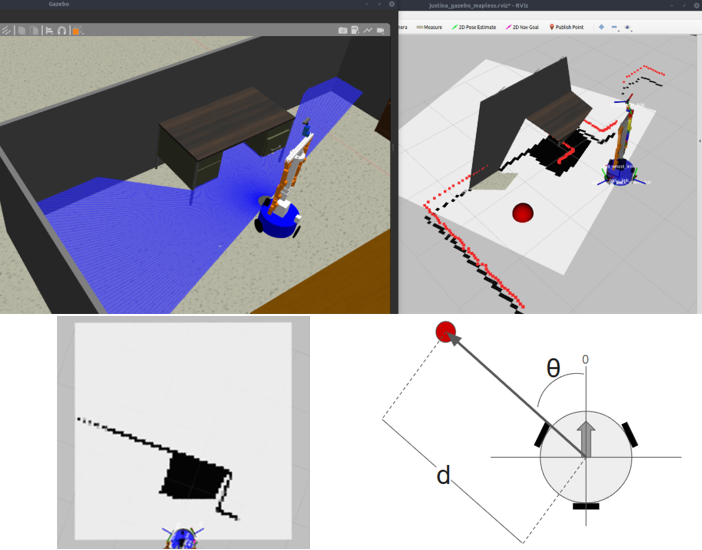
\includegraphics[width=0.55\textwidth]{images/input_matrix.png}
\caption{Local environment signals: Local Obstacle Matrix (bottom left) and relative position vector of the target (bottom right).}\label{fig:input_signal}
\end{figure}

We aim to build a navigation system where the robot requires only information about free and occupied space in its immediate surroundings. The Local Obstacle Matrix (LOM) is a small occupancy grid obtained from the LiDAR sensor and a 2D projection of a point cloud, which are used to generate a representation of the perceived obstacles (see Subsection~\ref{subsec:inputs}); the LOM covers a square area in front of the robot. The target vector $(d, \theta)$ represents the relative position of the goal with respect to the robot's frame. These variables are the distance and angle in polar coordinates of the goal point. In Figure~\ref{fig:input_signal}, the target vector and the LOM generation process are shown. Both serve as inputs to the proposed neural network architectures, and the outputs consist of velocity commands in the form $(v_x, v_y, \omega)$, where $v_x$ and $v_y$ are the linear velocities along the robot's $x$ and $y$ axes, respectively, and $\omega$ is the angular velocity around the robot's vertical axis. In Figure~\ref{fig:gen_sch} a general scheme of the navigation behavior system is presented.

\begin{figure}[htbp]
    \centering
    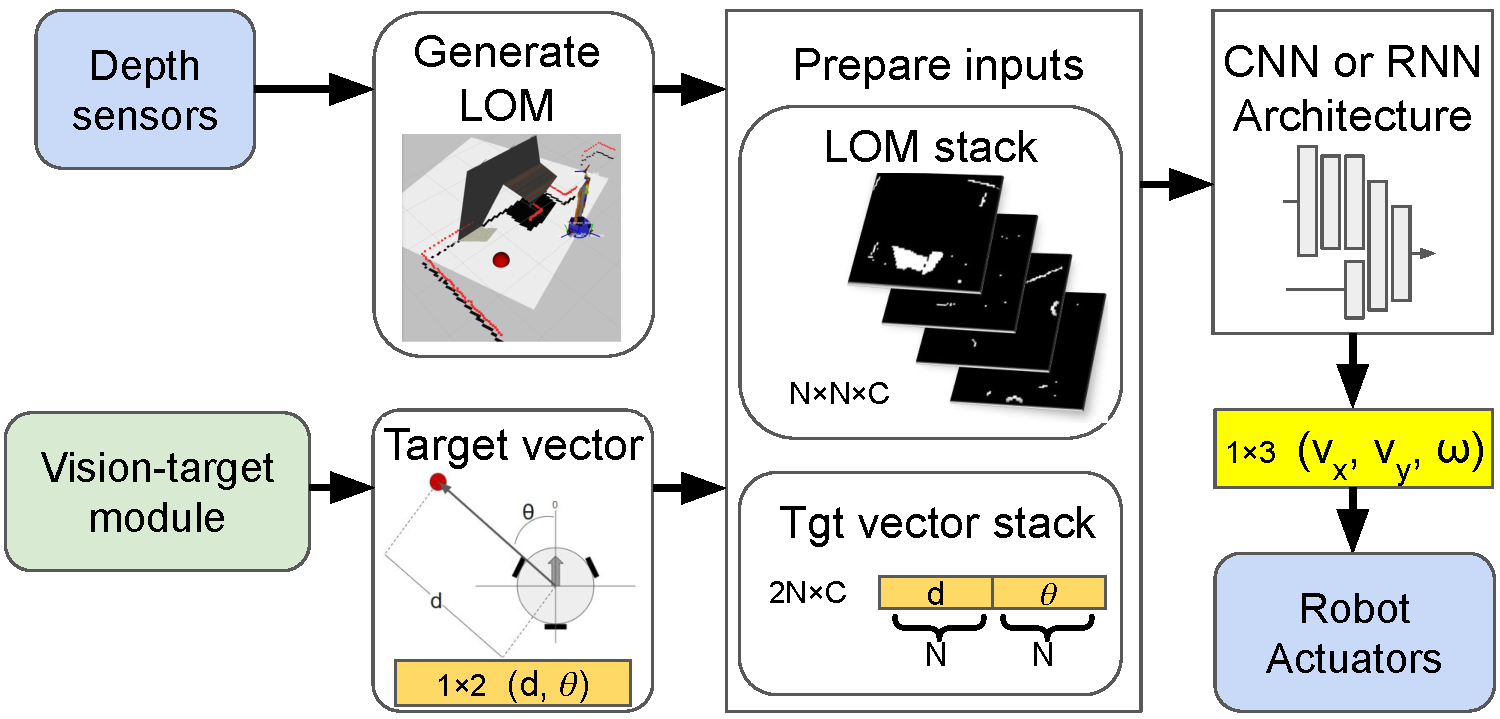
\includegraphics[width=0.8\textwidth]{images/General_diagram.pdf}
    \caption{General navigation behavior system scheme.}
    \label{fig:gen_sch}
\end{figure}

\subsection{The Binary Local Obstacle Matrix (LOM)} \label{subsec:inputs}

The binary LOM can be generated using various depth sensors or estimators, such as RGB-D cameras, ultrasonic sensors, LiDAR, 3D point clouds, or neural network–based depth estimators. In this work, we use two complementary sensors: an RGB-D camera mounted on the robot's head provides point cloud data, while a 2D LiDAR sensor located on the robot's base provides laser scans. We fuse both sources to build a richer representation of the surroundings. The LOM is an $N \times N$ matrix at ground level, where each cell encodes the presence of an obstacle. For each cell, we project the corresponding 3D points from the point cloud and also integrate the LiDAR readings that fall into that cell. The final value of a cell is set to 100 if either sensor detects an obstacle, and 0 otherwise.

% LOM encoding comparison.
\textcolor{red}{The LOM is treated as a single-channel binary image. Its two values represent free and occupied space; changing the occupied-cell value modifies the numerical input scale without changing the obstacle geometry. To select the occupied-cell value, we compared the 0/1, 0/100, and 0/255 encodings using RNN models trained with different random seeds and the same dataset and training hyperparameters. Among the selected models, 0/100 achieved the lowest average validation mean squared error (MSE), 0.075609, compared with 0.084249 for 0/1 and 0.085079 for 0/255.}

\textcolor{red}{To assess the use of obstacle information, we permuted complete LOM sequences between validation samples while keeping the target vectors, reference velocity commands, and model weights fixed. The MSE increased by 74.29\% with 0/100, compared with 4.80\% with 0/1 and 59.96\% with 0/255. This sensitivity indicates that the 0/100 models use obstacle information together with the target vector to predict velocity commands.}

\textcolor{red}{In navigation tests for this encoding comparison, with obstacles concentrated on the left or right, the goal was reached without collisions in 70\% of the cases with 0/100, compared with 10\% with 0/1 and 50\% with 0/255. These results support the selection of 0/100 for the evaluated configuration.}

\subsection{Proposed CNN Architecture} \label{subsec:cnn_arq}

Convolutional neural networks (CNNs) \citep{krizhevsky2012imagenet} are widely used in computer vision tasks. The early layers of a neural network are typically convolutional and are used to extract features from the input data. Adding several layers increases the network’s level of abstraction, and the number of layers depends on the complexity of the dataset. CNNs exhibit a certain degree of invariance to translation, scaling, and input distortions, which contributes to their robustness. Each convolutional layer has a set of filters, or channels, that determine the depth of the generated feature map. Convolutions effectively preserve spatial relationships; however, to provide some ability to learn spatio-temporal features, we propose using a sequence of binary images stacked as channels in the main input of our architectures.

Our neural network has two inputs: the first is our binary LOM, and the second is an auxiliary input (the target vector). The auxiliary input is provided at a later stage because we first want to extract features from the LOM independently. The first input can be interpreted as an $N\times N$ image. To incorporate temporal information into the learning process, $C$ consecutive frames are provided to the network, stacked as channels forming a single input tensor of dimensions$N\times N \times C$. Each of these $C$ frames has an associated target vector$(d, \theta)$, which together form the auxiliary input sequence. Samples are stored sequentially to preserve the frame order. During data selection in the training phase, packets of $C$ channels are obtained before shuffling the samples. Thus, each sample is not a single image but rather a sequence of $C$ frames, this approach accelerates training convergence.

The proposed architecture consists of three convolutional layers with ReLU activation; to reduce spatial dimensionality, max pooling is applied to the second and third layers. On the second layer, batch normalization is applied to stabilize learning. The resulting feature map is flattened, producing a high-dimensional feature vector that encodes the spatial and temporal information from the LOM sequence. This vector is then concatenated with the auxiliary input (the target vector) in a late-fusion fashion \citep{brenner2023rgbdt} (specifically, feature-level fusion), where the two information streams are processed independently before being combined at a deeper stage of the network. Because the flattened feature map from the convolutional layers has dimensionality proportional to $N^2$, whereas the target vector $(d, \theta)$ has only two components, direct concatenation would disproportionately weight the LOM-derived features. To prevent the auxiliary input from being marginalized during training and ensure its contribution remains relevant for the final regression task, the vector $(d, \theta)$ is replicated $N$ times, as expressed in Equation \eqref{eq:repeated_target}. The resulting concatenated vector is then passed through two fully connected (FC) layers (each with dropout). The output layer consists of three $\tanh$ neurons that provide the learned three control robot velocities $(v_x, v_y, \omega)$. Full architecture is shown in Figure~\ref{fig:CNN_arch}.

\begin{equation}
\text{rep\_tgt} = 
\big[\, d_{i,c}, \theta_{i,c} \,\big]_{i=1,\dots,N;\, c=1,\dots,C} 
\in \mathbb{R}^{2NC}
\label{eq:repeated_target}
\end{equation}

For the specific implementation, we use $N = 80$ and $C = 4$, resulting in an input tensor of size $80 \times 80 \times 4$. Three convolutional layers with $3 \times 3$ kernels (16, 32, and 8 filters) and ReLU activation, followed by max pooling ($5 \times 5$, stride 3), produce a flattened feature vector of $288$ dimensions. The target vector replicated $80$ times ($160$ dimensions) is concatenated, forming a $448$ dimensional input to two fully connected layers (120 and 80 neurons) with dropout rates of $0.2$ and $0.15$, respectively. The output layer uses $\tanh$ activation to produce velocity commands $(v_x, v_y, \omega)$, normalized to $[-1, 1]$.

\begin{figure}[htbp]
\centering
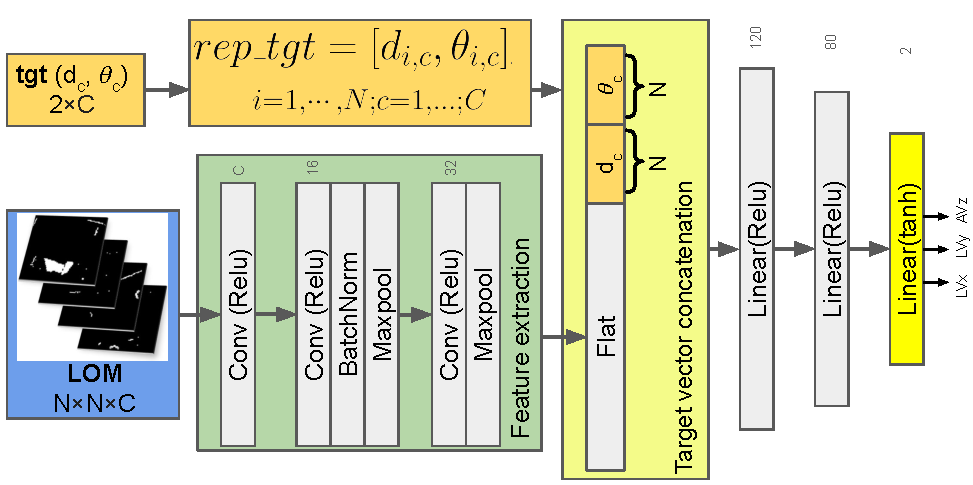
\includegraphics[width=\columnwidth]{images/CNN_arch_FE.pdf}
\caption{CNN architecture with $C$ sequential frames and targets; target vector is replicated $N$ times and concatenated with extracted features.}\label{fig:CNN_arch}
\end{figure}

\subsection{Proposed RNN Architecture}\label{subsec:rnn_arq}

Recurrent Neural Networks (RNNs) gained prominence in the 1990s due to their ability to retain information from previous inputs through feedback connections \citep{elman1990finding}. Their feedback connections allow an inherent capacity for temporal memory, making them particularly well-suited for tasks in which temporal order and context are critical, such as language processing, music analysis, and robotics \citep{Danilorecurrent2001}. Applications of RNNs include speech recognition, machine translation, musical sequence generation, and autonomous decision-making in robots and self-driving vehicles.

To maintain compatibility within our system, our recurrent neural network architecture shares the same input and output structure as the previous CNN architecture. The first layer is a convolutional layer with max pooling to reduce feature dimensionality. The resulting feature channels are flattened separately and concatenated with the target vector $(d, \theta)$ in a different way than in the CNN. Instead of obtaining a single vector by flattening all features and concatenating it with a repeated target vector, we obtain $C$ flattened feature vectors, each concatenated with its respective repeated target vector. After concatenation, these $C$ vectors serve as input to our recurrent block, which consists of four simple recurrent layers (with tanh activation). Each RNN cell (see Figure~\ref{fig:RNN_cell}) reuses hidden state information, and the cells are interconnected in a many-to-one configuration. The output from the recurrent block is a feature vector that passes through the three fully connected (FC) layers, which generate the control signals. The full architecture is shown in Figure~\ref{fig:RNN_arch}.

Unlike the CNN, the RNN model operates with $N = 80$ and $C = 2$, producing an input tensor of size $80 \times 80 \times 2$. A single convolutional layer with 8 filters ($3 \times 3$ kernels) and ReLU activation, followed by max pooling ($7 \times 7$, stride 3), produces a flattened feature vector of $4608$ dimensions per channel. The target vector replicated $80$ times ($160$ dimensions) is concatenated per channel, forming a $4768$ dimensional input vector for each of the $C$ channels. These vectors are processed by a recurrent block with four RNN layers, each with $350$ hidden units and tanh activation, operating in a many-to-one configuration. The recurrent block outputs a $350$ dimensional feature vector from the final time step, which is then passed through three fully connected layers (120, 80, and 3 neurons) with dropout (0.2 and 0.15) and $\tanh$ activation to produce the velocity commands $(v_x, v_y, \omega)$, normalized to $[-1, 1]$.

\begin{figure}[htbp]
\centering
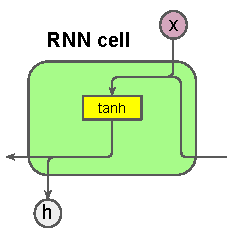
\includegraphics[width=0.3\columnwidth]{images/RNN_cell.pdf}
\caption{An RNN cell implemented in our recurrent block.}\label{fig:RNN_cell}
\end{figure}
% TODO: evaluar explicación
%\caption{\textcolor{red}{An RNN cell implemented in our recurrent
%block. The input $x$ is the concatenated feature and target vector
%in the first recurrent layer, or the preceding layer's output
%in subsequent layers. The variable $h$ denotes the hidden state.}}

\begin{figure}[htbp]
\centering
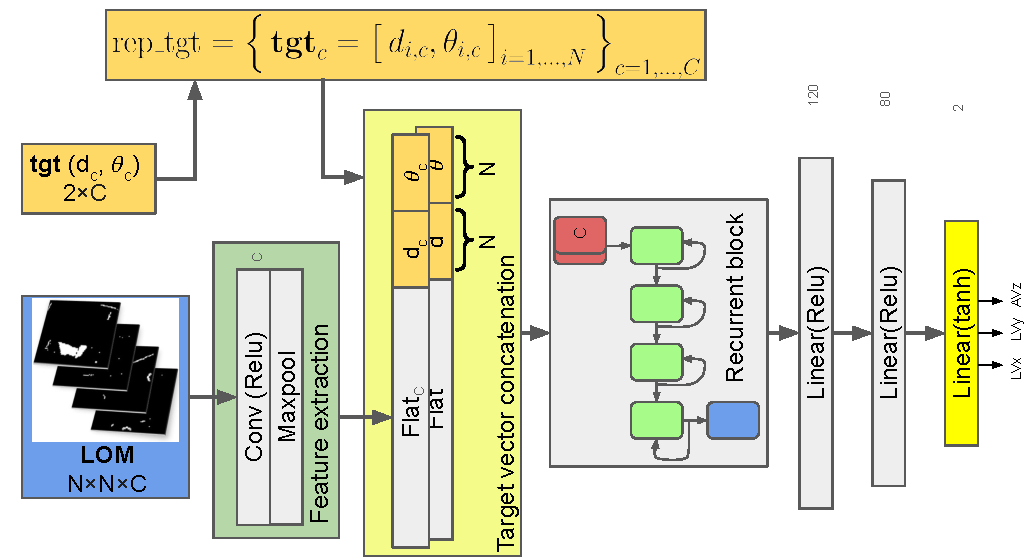
\includegraphics[width=\columnwidth]{images/RNN_arch_FE.pdf}
\caption{RNN architecture. The recurrent block receives $C$ input vectors, each obtained by concatenating a feature vector with its corresponding repeated target vector $(d, \theta)$.}\label{fig:RNN_arch}
\end{figure}

\section{Training of Neural Network Architectures}\label{sec:training}

Our proposed neural network models—the CNN and RNN (see Subsections~\ref{subsec:cnn_arq} and~\ref{subsec:rnn_arq})—employ supervised learning and therefore require labeled data. Because the network outputs are continuous velocity commands, the learning task is formulated as a regression problem. We train the models by minimizing the mean squared error (MSE) between the predicted velocities and the ground-truth commands recorded during data collection. The hyperparameters used for training both models are summarized in Table~\ref{tab:hyperparams}.

For the experiments, six different environments were generated using a custom generator developed by us (see Subsection~\ref{subsec:random_map}). Three of these environments were used for data collection and are therefore considered "known" environments, while the remaining three are treated as "unknown" environments. Data collection was carried out using a script that validates and stores the labels while the robot navigates through the environment toward randomly selected target objectives inside the navigable area, as described in Subsection~\ref{subsec:Dataset}. Navigation can be executed either manually by a human operator (without requiring a map) or autonomously through a navigation system. In our case, to avoid introducing bias, we employed our PNS (see Subsection~\ref{subsec:pumas_nav}). 

\begin{table}[htbp]
\centering
\begin{tabular}{|l|c|c|}
\hline
\textbf{Parameter} & \textbf{CNN Value} & \textbf{RNN Value} \\
\hline
$C$ (stacked frames) & 4 & 2 \\
Batch size & 8 & 3 \\
Learning rate & $1 \times 10^{-4}$ & $6 \times 10^{-4}$ \\
Epochs & 20 & 20 \\
Patience & 5 & 5 \\
Optimizer & Adam & Adam \\
Loss function & MSE & MSE \\
Convolutional layers & 3 & 1 \\
Filters & 16, 32, 8 & 8 \\
RNN hidden units & — & 350 \\
RNN layers & — & 4 \\
\hline
\end{tabular}
\vspace{2.5pt}
\caption{Hyperparameters for CNN and RNN training.}
\label{tab:hyperparams}
\end{table}

\subsection{The Pumas Navigation System (PNS)}\label{subsec:pumas_nav}

The PNS \citep{contreras2025b} is the standard map-based navigation system in our robots. PNS implements the A* algorithm with a cost function that evaluates collision risk during path planning; calculated paths have a configurable tradeoff between safety and distance. A particle filter with ROS implementation is used for localization and mapping. A finite state machine coordinates obstacle avoidance behavior using potential field and general planning.

\subsection{Random Map Generator} \label{subsec:random_map}

% Map generator.
\textcolor{red}{We developed a Blender-based random map generator that subdivides a rectangular floor plane into rooms. The subdivision configuration parameter $SC$ is intended to increase structural complexity by favoring more subdivisions as its value increases. The number of rooms depends jointly on the floor area and a random factor sampled between $SC$ and $SC^2$; therefore, $SC=3$ does not imply exactly three rooms. Map dimensions are sampled separately within configured ranges. Random sampling and variations in cut positions introduce diversity in room counts, sizes, and shapes, including among environments generated with the same $SC$. The generated meshes are imported into the simulator, where furniture is added separately to obtain plausible indoor arrangements.}

% Original experimental configuration.
\textcolor{red}{For the six environments used in the original navigation experiments (E1--E6), map dimensions ranged from $5$ to $10$ meters along both axes. The generator was configured with $SC=2$, and the selected layouts contained two rooms. Furniture was added separately, with $10$--$25$ items per room. These counts describe the selected scenarios rather than fixed outputs of the subdivision parameter.}

\textcolor{red}{We used the same generator to produce 30 environments (E1–E30) with different layouts, physical sizes, and values of the subdivision parameter $SC$ (SC2--SC30) for the analysis of environmental similarity. The navigation experiments reported in this paper were conducted in six environments (E1–E6), reflecting the scope of the original evaluation. The 30-environment analysis characterizes geometric differences across a broader set of maps; it does not, by itself, establish a relationship between the similarity metric and navigation performance.}

% Room subdivision.
\textcolor{red}{At each subdivision step, the algorithm selects either a random face or the largest available face and applies a cut with a random edge-slide offset between $-0.8$ and $0.8$. This introduces additional variation in room shapes and proportions.}

The resulting geometric maps, shown in Figure~\ref{fig:maps}, illustrate the occupied space in each environment; a 1 m grid is overlaid on each map to provide spatial scale. Only the E1--E3 maps were used by our PNS to collect training data, as this map-based system requires a geometric map for operation. The collected dataset was then used to train the neural networks. Importantly, the neural networks themselves \textbf{\textcolor{red}{do not use global geometric maps during execution}}; they operate solely on the LOM and target vector inputs, and data could also have been collected by manually operating the robot, as described in Subsection~\ref{subsec:Dataset}.

\begin{figure}[htbp]
\centering
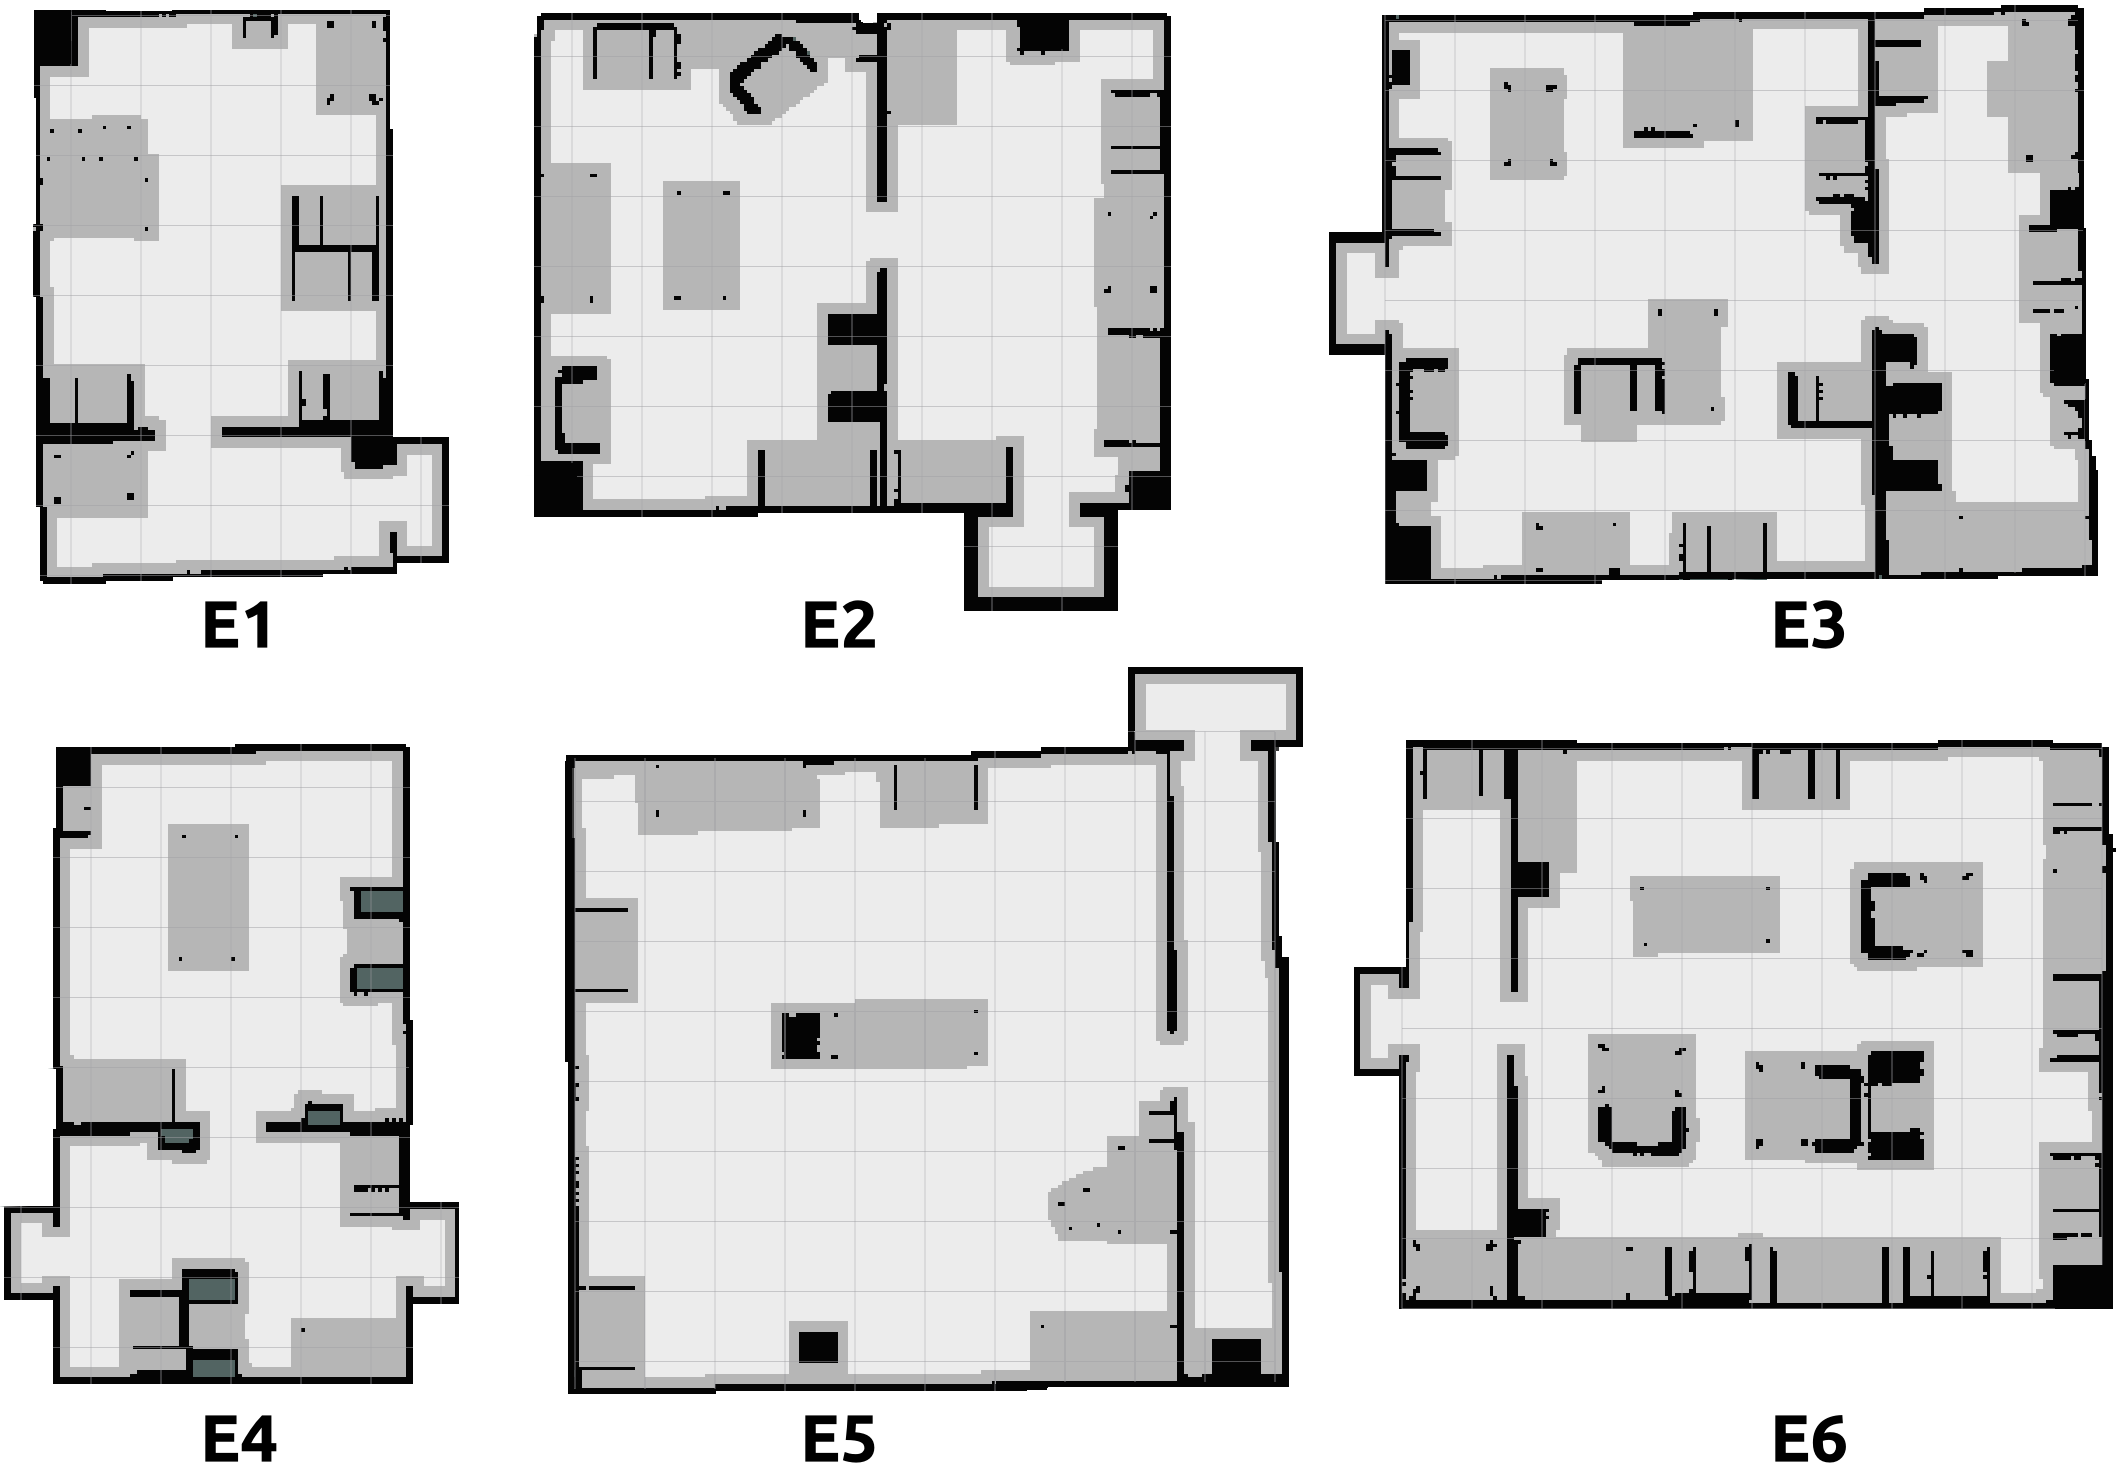
\includegraphics[width=\columnwidth]{images/maps.png}
\caption{Randomly generated environments.}\label{fig:maps}
\end{figure}

\subsection{Dataset Collection}\label{subsec:Dataset}

The curriculum learning approach \citep{DBLP:journals/corr/abs-2101-10382} improves model efficiency during training by gradually increasing task difficulty. Following this principle, we initially trained the model in a single empty room to allow it to learn basic movements (turning left and right, moving forward and backward) for navigating toward a given target. Subsequently, data collection was expanded to include samples of the robot moving between rooms interconnected by a door. Unfortunately, the resulting dataset presented challenges, leading to unstable behaviors. In many cases, the trajectories followed by the trained model formed spiral paths instead of moving directly toward the target. We concluded that in empty environments, the predominantly zero values in the LOM prevented the model from effectively associating appropriate control commands with similar inputs.

To address this issue, training and testing data were automatically captured by a script using the PNS (see Figure~\ref{fig:data_collect} and Subsection~\ref{subsec:pumas_nav}), which enables the robot to navigate within an environment for data acquisition. The corresponding geometric maps were required for the PNS only and not for other purposes. The script loads the occupancy grid map of the current environment, extracts all free cells, and stores their coordinates in a temporary array. At each step, it randomly selects a point from this array as the new target, ensuring that the goal always lies in free space. To maintain consistency in the collected samples—so that trajectories have similar length and difficulty—targets are constrained to lie within a 3.5 m radius of the robot’s current position. To eliminate the risk of collision, which would produce erroneous sensor readings and control commands, the PNS employs potential fields with lateral movements (linear velocity $y$). A total of 3,880 samples were collected across E1, E2, and E3 (see Figure~\ref{fig:maps}).

To incorporate temporal information—particularly for the CNN model—the dataset is recorded and organized as sequences of $C$ consecutive samples collected during navigation toward a designated target. Each sample consists of a pair comprising the LOM and target vector as input, and the corresponding command velocity sequence as output. In other words, we store each training sample as a sequence of $C$ simple samples, where each input pair $(\mathbf{LOM}, \mathbf{tgt})$ is associated with its corresponding output velocity vectors $\mathbf{v}$. Formally, the label for sample $i$ is defined as

\begin{equation}
\text{Label}^{(i)} = \big((\mathbf{LOM}^{(i)}, \mathbf{tgt}^{(i)}), \mathbf{v}^{(i)}\big)
\label{train_labels}
\end{equation}

where:\\
$\text{LOM}^{(i)} \in \{0, 100\}^{N \times N \times C}$: sequence of $C$ binary LOM frames for sample $i$.\\
$\mathbf{tgt}^{(i,c)} = (d^{(i,c)}, \theta^{(i,c)}) \in \mathbb{R}^{2}$: sequence of $C$ target vectors for sample $i$.\\
$\mathbf{v}^{(i,c)} = (v_x^{(i,c)}, v_y^{(i,c)}, \omega^{(i,c)}) \in \mathbb{R}^{3}$: sequence of $C$ command vectors for sample $i$, where $v_x$ and $v_y$ are the linear velocities along the robot's $x$ and $y$ axes, respectively, and $\omega$ is the angular velocity around the robot's vertical axis.\\
$N$: LOM pixel size.

We tested multiple hyperparameter combinations and selected those that stabilized training and produced consistent results. For our CNN, we selected a batch size of 8, meaning that each training batch consists of 8 samples, with each sample corresponding to a 4-channel ($C = 4$) LOM array of consecutive frames. For the RNN model, we use a batch size of 3, with each sample corresponding to a 2-channel ($C= 2$) LOM array. The LOM is a binary N$\times$N pixel matrix encoding a squared area in front of the robot. \textcolor{red}{A $4\times4$ m region works well in different scenarios.} Using a larger area may reduce training stability, while a smaller area reduces the capability to detect obstacles and thus increases the collision risk. The size of N in pixels is 80 and is defined by the resolution of the local occupancy projection calculated as follows: \textcolor{red}{$N=m\,\mathrm{Res}$, where $m$ is the side length in meters and
$\mathrm{Res}$ is the resolution expressed in cells per meter.
With $m=4$ m and $\mathrm{Res}=20$ cells/m, $N=80$.}

The underlying control loop of the PNS, which includes the potential fields for obstacle avoidance, operates at 30 Hz. While the robot navigates to each new target, the input signals (LOM and target vector, described in Subsection~\ref{subsec:inputs}) and their corresponding labels $\mathbf{v} = (v_x, v_y, \omega)$ are recorded at 5 Hz. This sampling rate ensures that consecutive samples are sufficiently different, preventing redundant samples that would add little information to the learning process. It also captures the net effect of the potential fields rather than momentary fluctuations, ensuring the dataset reflects meaningful navigation behavior instead of high‑frequency noise. The data are stored in a Python dictionary as an .npz file while at least one component of data\_Y exceeds 0.1; otherwise, the sample is discarded (i.e., when the robot remains stationary).

\begin{figure}[htbp]
\centering
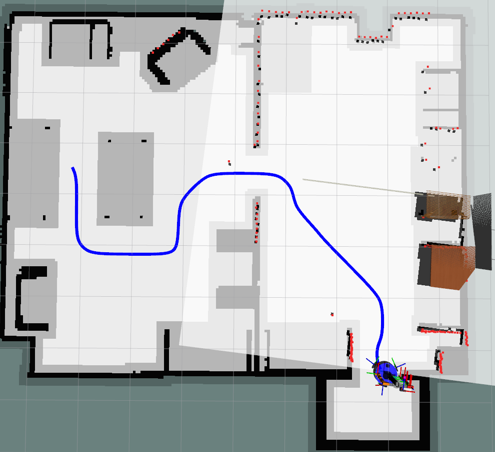
\includegraphics[width=0.4\columnwidth]{images/data_collection.png}
\caption{Automated data collection process using the PNS.}\label{fig:data_collect}
\end{figure}

\begingroup
\color{red}
\section{Environment Similarity Metric}\label{sec:metric_definition}

The core hypothesis of this work is that the geometric structure of an environment dictates the difficulty of zero-shot generalization for a mapless navigation policy. To quantify this structural difference, we model each environment as a discrete probability distribution of obstacles and compute the optimal transport cost between them.

\subsection{Definition of the Metric}\label{subsec:metric_def}
\textbf{Environment Representation.}

Let an environment \(\mathcal{E}\) be represented by a binary occupancy grid \(\mathcal{M}\), where cells are either free or occupied. We extract the set of metric coordinates of all occupied cells, denoted as \(\mathcal{P} = \{p_i = (x_i, y_i)\}_{i=1}^{|\mathcal{P}|}\), where \(x_i\) and \(y_i\) are expressed in meters relative to a common global origin. To ensure the metric is invariant to the absolute placement of the map within the grid, we align all maps by their geometric center prior to extraction.

Since a full occupancy grid contains tens of thousands of points, we treat the environment as an empirical probability measure \(\mu\) over its occupied cells:

\begin{equation}
    \mu = \frac{1}{|\mathcal{P}|} \sum_{i=1}^{|\mathcal{P}|} \delta_{p_i}
\end{equation}

where \(\delta_{p_i}\) is the Dirac delta function at position \(p_i\). To make the computation tractable for high-resolution grids, we subsample a fixed number \(n_p\) of points uniformly at random from each map, where \(n_p\) is referred to as the \emph{sampling density}. Throughout this work we use \(n_p=4000\) points per environment, yielding a sparse empirical distribution \(\hat{\mu}\) over the subsampled cells.

\textbf{Wasserstein Distance and Sinkhorn Regularization.}

Given two environments \(\mathcal{A}\) and \(\mathcal{B}\) with empirical distributions \(\hat{\mu}_A\) and \(\hat{\mu}_B\), we quantify their structural dissimilarity using an entropy-regularized optimal transport cost related to the 1-Wasserstein distance (Earth Mover's Distance). This cost quantifies the effort required to transport the obstacle distribution of \(\mathcal{A}\) into that of \(\mathcal{B}\). 

To compute this efficiently while maintaining differentiability and numerical stability, we adopt the entropy-regularized optimal transport formulation (Sinkhorn distance). Let \(\mathbf{D} \in \mathbb{R}^{n_p \times n_p}\) be the cost matrix, where \(D_{ij} = \|p_i - p_j\|_2\) is the Euclidean distance between points \(p_i \in \mathcal{A}\) and \(p_j \in \mathcal{B}\). The Sinkhorn distance is defined as:

\begin{equation}
    d_{\text{Sinkhorn}}(\mathcal{A}, \mathcal{B}) = \min_{\boldsymbol{\Gamma} \in \Pi(\hat{\mu}_A, \hat{\mu}_B)} \sum_{i,j} \Gamma_{ij} D_{ij} - \lambda H(\boldsymbol{\Gamma})
    \label{eq:sinkhorn}
\end{equation}

where \(\Pi(\hat{\mu}_A, \hat{\mu}_B)\) is the set of all transportation plans (joint probabilities with marginals \(\hat{\mu}_A\) and \(\hat{\mu}_B\)), \(H(\boldsymbol{\Gamma}) = -\sum_{i,j} \Gamma_{ij} \log \Gamma_{ij}\) is the entropy of the transport plan, and \(\lambda = 0.001\) is the entropic regularization parameter. A smaller \(\lambda\) yields a result closer to the exact EMD, but requires more iterations to converge. We use \(\lambda = 0.001\) with a maximum of 200 iterations.

\textbf{Global Scale Normalization.}

To ensure that the metric values are interpretable and independent of the absolute scale of the dataset, the cost matrix is normalized by the maximum pairwise distance across all sampled points in the dataset, denoted as \(s_{\text{global}}\). This normalization bounds the Wasserstein distances to the range \([0, 1]\), allowing direct comparison across different datasets and preventing numerical overflow during the Sinkhorn iterations.

\textbf{Bootstrap Averaging.}

Because the empirical distributions depend on the random subsampling of \(n_p\) points, a single distance computation is subject to sampling noise. To obtain a robust estimate, we perform \(B=5\) independent bootstrap resamples. The final reported distance \(\hat{d}(\mathcal{A}, \mathcal{B})\) is the mean over the \(B\) runs, and the standard deviation across these runs summarizes resampling variability; it is not, by itself, a confidence interval.

\subsection{Validation of the Metric}\label{sec:metric_validation}

To characterize the proposed environment similarity metric, we evaluated all 30 procedurally generated environments, yielding 435 unique pairwise comparisons. The analysis examines numerical stability under point subsampling and sensitivity to physical scale; it does not yet validate the metric as a predictor of navigation performance. 

\textbf{Statistical Robustness and Dynamic Range.}

As detailed in Table \ref{tab:metric_validation_stats}, the pairwise distances range from \(0.0337\) (nearly identical layouts) to \(0.1733\) (highly distinct topologies), providing a dynamic range of \(5.14\times\). The ranked pairs in Tables \ref{tab:most_similar} and \ref{tab:most_distinct} illustrate the range of structural differences measured across the 30 environments. Furthermore, the metric is highly stable: the mean coefficient of variation (CV) across all pairs is \(1.20\%\) over 5 bootstrap resamples with a sampling density of \(n_p=4000\) points per environment. To evaluate the sensitivity to point cloud density, we performed a cross-validation using \(n_p=2000\) points. The rank correlation between both configurations exceeded \(0.99\), and the dynamic range remained virtually unchanged (\(5.05\times\)). While \(n_p=2000\) is computationally sufficient, we report the \(n_p=4000\) configuration for maximum statistical fidelity.

\textbf{Scale Sensitivity vs. Topological Similarity.}

A critical challenge for similarity metrics is distinguishing between visual topological similarity and physical metric scale. To address this, we designed a controlled reference case. Environment E07 was generated with the exact same furniture layout, angles, and relative positions as E05, but scaled to a larger physical dimension. 

As shown in Table \ref{tab:scale_control}, despite their visual similarity, the metric yields a distance of \(0.1185 \pm 0.0007\) between E05 and E07, placing them in the top 15\% of most dissimilar pairs. In contrast, environments with different topologies but identical physical scales (e.g., E05 and E03) yield a distance of only \(0.0472\). This indicates that the metric is sensitive to physical distances between obstacles (in meters), in addition to layout differences. Whether these distances predict navigation generalization requires a separate analysis against navigation outcomes. A policy trained in a smaller room may fail in a visually identical but larger room due to different spatial constraints and required trajectory lengths.

\begin{table}[htbp]
\centering
\caption{Statistical summary of the 435 pairwise Wasserstein distances across 30 environments. \(n_p\) denotes the sampling density (points per environment).}
\label{tab:metric_validation_stats}
\begin{tabular}{lcc}
\toprule
\textbf{Metric} & \textbf{Configuration \(n_p=4000\)} & \textbf{Configuration \(n_p=2000\)} \\
\midrule
Distance range & \(0.0337 - 0.1733\) & \(0.0349 - 0.1762\) \\
Dynamic range (max/min) & \(5.14\times\) & \(5.05\times\) \\
Mean Coefficient of Variation (CV) & \(1.20\%\) & \(1.75\%\) \\
Spearman rank correlation & \multicolumn{2}{c}{\(> 0.99\)} \\
\bottomrule
\end{tabular}
\end{table}
\begin{table}[htbp]
\centering
\caption{Controlled scale validation. E05 and E07 share identical visual layouts but differ in physical scale. Distances are reported as mean \(\pm\) standard deviation. \(n_p\) denotes the sampling density.}
\label{tab:scale_control}

\begin{tabular}{llcc}
\toprule
\textbf{Pair} & \textbf{Condition} & \textbf{Distance (\(n_p=4000\))} & \textbf{Distance (\(n_p=2000\))} \\
\midrule
E05 vs. E03 & Same scale, diff. layout & \(0.0472 \pm 0.0006\) & \(0.0481 \pm 0.0002\) \\
E05 vs. E07 & \textbf{Diff. scale, same layout} & \(\mathbf{0.1185 \pm 0.0007}\) & \(\mathbf{0.1192 \pm 0.0010}\) \\
E05 vs. E10 & Diff. scale, diff. layout & \(0.1733 \pm 0.0006\) & \(0.1762 \pm 0.0017\) \\
\bottomrule
\end{tabular}
\end{table}

\textbf{Ranked environment pairs.} Tables~\ref{tab:most_distinct} and~\ref{tab:most_similar} report the ten most structurally distinct and the ten most structurally similar pairs, respectively, according to the mean normalized distance computed with \(n_p=4000\) points per environment. The reported \(\sigma\) is the standard deviation across the five resampling runs.

\begin{table}[htbp]
\centering
\caption{Top-10 most structurally distinct environment pairs.}
\label{tab:most_distinct}
\begin{tabular}{clcc}
\toprule
\textbf{Rank} & \textbf{Pair} & \textbf{Distance ($\hat{d} \pm \sigma$)} \\
\midrule
1 & E05 vs E10 & $0.1733 \pm 0.0006$ \\
2 & E10 vs E28 & $0.1688 \pm 0.0016$ \\
3 & E05 vs E09 & $0.1655 \pm 0.0012$ \\
4 & E01 vs E28 & $0.1634 \pm 0.0021$ \\
5 & E09 vs E28 & $0.1612 \pm 0.0018$ \\
6 & E04 vs E28 & $0.1602 \pm 0.0015$ \\
7 & E07 vs E28 & $0.1586 \pm 0.0028$ \\
8 & E05 vs E23 & $0.1488 \pm 0.0006$ \\
9 & E05 vs E19 & $0.1451 \pm 0.0012$ \\
10 & E01 vs E05 & $0.1444 \pm 0.0012$ \\
\bottomrule
\end{tabular}
\end{table}
\label{tab:most_distinct}


\begin{table}[htbp]
\centering
\caption{Top-10 most structurally similar environment pairs.}
\label{tab:most_similar}
\begin{tabular}{clcc}
\toprule
\textbf{Rank} & \textbf{Pair} & \textbf{Distance ($\hat{d} \pm \sigma$)} \\
\midrule
1 & E19 vs E25 & $0.0337 \pm 0.0002$ \\
2 & E01 vs E04 & $0.0350 \pm 0.0003$ \\
3 & E21 vs E29 & $0.0416 \pm 0.0011$ \\
4 & E18 vs E20 & $0.0419 \pm 0.0012$ \\
5 & E16 vs E29 & $0.0444 \pm 0.0008$ \\
6 & E22 vs E27 & $0.0461 \pm 0.0004$ \\
7 & E03 vs E05 & $0.0472 \pm 0.0006$ \\
8 & E09 vs E19 & $0.0480 \pm 0.0008$ \\
9 & E15 vs E26 & $0.0484 \pm 0.0005$ \\
10 & E02 vs E14 & $0.0498 \pm 0.0009$ \\
\bottomrule
\end{tabular}
\end{table}
\label{tab:most_similar}

\endgroup

\section{Experimental Setup}\label{sec:Experiments}

Once our neural network models were trained, the robot was placed in environments E1 through E6. Regardless of its initial position (no localization is required), a target point was randomly selected for navigation. The trained model waits for $C$ consecutive frames as input to perform inference, stacking the LOM and target vector as depicted in Figure~\ref{fig:gen_sch}. The output of the trained model consists of the velocity commands $(v_x, v_y, \omega)$ that our robot must command to its actuators. Often, the robot demonstrated the ability to evade dynamic obstacles.\textcolor{red}{The navigation policy used this relative target vector and the LOM sequence, without requiring localization within a global geometric map.}

Table~\ref{tab:map_tasks} summarizes the use of environments for training (tuning, configuring) and testing across maps E1 to E6.

\begin{table}[htbp]
\centering
\begin{tabular}{|l|c|c|c|c|c|c|}
\hline
\textbf{Used for / Map} & \textbf{E1} & \textbf{E2} & \textbf{E3} & \textbf{E4} & \textbf{E5} & \textbf{E6} \\
\hline
Training CNN               &  x  &  x  &  x  &     &     &     \\
\hline
Training RNN               &  x  &  x  &  x  &     &     &     \\
\hline
PF Constant Tuning         &     &  x  &     &     &     &     \\
\hline
FSM Parameter Selection    &     &     &     &  x  &     &     \\
\hline
\textcolor{red}{PNS Reference / Parameter Selection} &  x  &     &     &     &     &     \\
\hline
CNN Testing                &  x  &  x  &  x  &  x  &  x  &  x  \\
\hline
RNN Testing                &  x  &  x  &  x  &  x  &  x  &  x  \\
\hline
PF Testing                 &  x  &  x  &  x  &  x  &  x  &  x  \\
\hline
FSM Testing                &  x  &  x  &  x  &  x  &  x  &  x  \\
\hline
\textcolor{red}{PNS Mismatched (map E1 in E4)} &     &     &     &  x  &     &     \\
\hline
\end{tabular}
\vspace{2.5pt}
\caption{Usage of environments for training (or configuring/tuning) and testing. An \texttt{x} indicates that the environment was used for that purpose. For the neural network models (CNN and RNN), environments E1–E3 are \textit{known} (used for training), while E4–E6 are \textit{unknown} (not seen during training). \textcolor{red}{For the PNS, E1 is the reference case with the correct map, and E4 is the mismatched-map case, where the map from E1 is used in E4.}}
\label{tab:map_tasks}
\end{table}

\subsection{Test of the Pumas Navigation System (PNS) in Known and Unknown Environments}\label{subsec:pns_test}

Traditional map-based navigation systems have been shown to outperform many mapless navigation techniques in previously known environments, where an updated map is provided. However, they lack the ability to generalize navigation when the environment suffers significant changes. This limitation is proven in the following experiment.

We start with environment E1 to navigate with our map-based PNS, using the corresponding map E1; this is the reference case, where the map matches the environment. As expected, the navigation performance was very high. In a second stage, we deployed our robot in environment E4, but using the map from E1 instead; this is the mismatched-map case, where the environment is unknown to the PNS and the available map is outdated. Considering some similarity in space between E1 and E4, and even though the PNS employs potential fields to obstacle avoidance, navigation performance drops drastically, and was unable to successfully navigate to a new target provided. The experiment highlights the need to remap every new unseen environment. The results are summarized in Table \ref{tab:nav_system}.

\begin{table}[htbp]
\centering
\begin{tabular}{|c|c|c|}\hline
    Navigation system & Env E1 with map E1 &  Env E4 with map E1 \\ \hline
    Reach the Target & 98\%  & 26\% \\ \hline
    Collisions & 0 & 26 \\ \hline
\end{tabular}
\vspace{2.5pt}
\caption{PNS tested in the known environment E1 with the correct map (reference case), and in the unknown environment E4 with the outdated map from E1 (mismatched-map case).}\label{tab:nav_system}
\end{table}

\subsection{Mapless Navigation Techniques Comparison}

All environments generated (see Subsection~\ref{subsec:random_map}) were used to test the navigation performance of each methodology, except for the map-based navigation system. \textcolor{red}{The PNS was evaluated in two conditions: E1 with the correct map (reference case) and E4 with the outdated map from E1 (mismatched-map case), as described in Subsection~\ref{subsec:pns_test}.} For the neural network models, E1, E2, and E3 were used to collect the dataset; thus, they are considered previously known environments, while E4, E5, and E6 are considered unknown. The finite state machine (FSM) was configured in advance in environment E4 to test its performance, whereas the parameters of the potential fields (PF) were tuned in E2. Consequently, E4 and E2 are considered previously known environments for the FSM and PF baselines, respectively.

\begin{figure}[htbp]
\centering
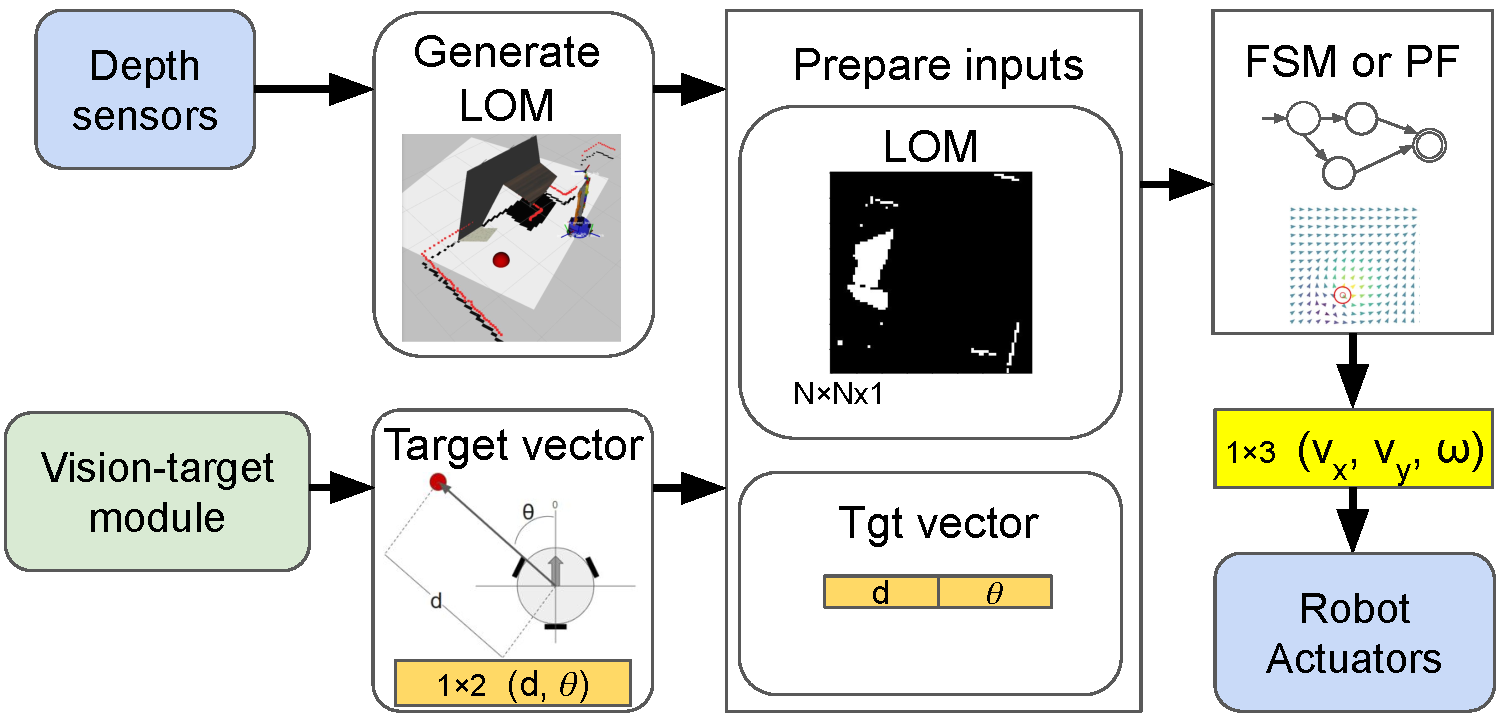
\includegraphics[width=0.8\columnwidth]{images/General_diagram_FSM-PF.pdf}
\caption{General navigation scheme describing the behavior of FSM and PF approaches.}
\label{fig:fsm-pf_sch}
\end{figure}

\begin{algorithm}
\caption{Pseudocode for the Finite State Machine (FSM) Baseline}
\label{alg:fsm_reactive}
\begin{algorithmic}[1]

\While{true}

    \If{no goal}
        \State Stop and wait for goal
    \Else
        \State Read $d, \theta$, lidar, occupancy

        \If{robot is within goal tolerance}
            \State Stop
        \ElsIf{front is free}
            \State Move toward the goal
        \Else
            \State $s \gets$ \Call{ChooseFreeSide}{lidar, occupancy}

            \If{$s \neq$ BLOCKED}
                \While{front blocked} 
                    \State Rotate toward free side $s$
                \EndWhile
            \Else
                \State Rotate to largest gap; move back
            \EndIf

            \State Move forward a short distance
        \EndIf
    \EndIf

\EndWhile

\vspace{0.2cm}
\hrule
\vspace{0.2cm}

\Function{ChooseFreeSide}{lidar, occupancy}
    \If{both sides free} \Return side with more space
    \ElsIf{left free} \Return LEFT
    \ElsIf{right free} \Return RIGHT
    \Else \Return BLOCKED
    \EndIf
\EndFunction

\end{algorithmic}
\end{algorithm}

\begin{figure}[htbp]
\centering
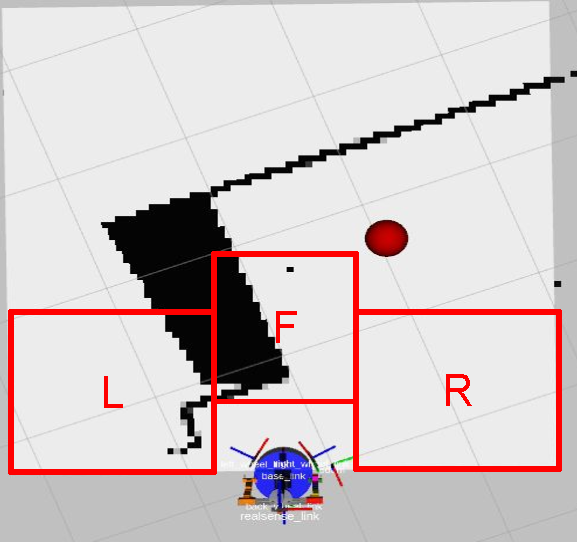
\includegraphics[width=0.4\columnwidth]{images/FSM_sensors.pdf}
\caption{Perception zones used by the FSM for obstacle detection: left (L), front (F), and right (R). The red-marked areas indicate the regions evaluated to determine free space and select evasion directions.}
\label{fig:fsm_obstacle}
\end{figure}

The finite state machine (FSM) baseline implements reactive obstacle avoidance using laser scans and a local occupancy grid; the general navigation scheme for its behavior is shown in Figure~\ref{fig:fsm-pf_sch}. The FSM evaluates three regions—left, front, and right—as illustrated in Figure~\ref{fig:fsm_obstacle}. Obstacle detection is performed by laser scan data, which provides distance measurements, and a local occupancy grid, which gives obstacle density in the robot's immediate vicinity. When an obstacle is detected, the FSM selects an evasion direction (left, right, or backward) based on free space availability. The front region is considered blocked if the occupancy grid shows any obstacle directly ahead. For side selection, the FSM checks both left and right using laser scans to identify free space. If both sides are blocked, the robot rotates toward the largest visible gap detected by the laser and moves backward to create space for maneuvering. If both sides are free, it selects the side with the largest continuous free space; if only one side is free, that side is chosen. When all regions are free, the robot rotates for a fixed duration toward the goal based on the initial target angle and moves forward before evaluating new sensor readings. The reactive navigation strategy implemented by the FSM is summarized in Algorithm~\ref{alg:fsm_reactive}.

In contrast to the rule-based FSM, the potential fields (PF) baseline follows the same general navigation scheme illustrated in Figure~\ref{fig:fsm-pf_sch}, using attractive and repulsive forces to generate velocity commands. The attractive force pulls the robot toward the goal, while repulsive forces push it away from obstacles detected by laser scans. The resultant force vector determines the robot's motion direction. The logic is detailed in Algorithm~\ref{alg:pf_reactive}.

\begin{algorithm}
\caption{Pseudocode for the Potential Fields (PF) Baseline}
\label{alg:pf_reactive}
\begin{algorithmic}[1]

\While{true}

    \If{no goal}
        \State Stop and wait for goal
    \Else
        \State Read target $(d, \theta)$, laser, occupancy

        \If{within goal tolerance}
            \State Stop
        \Else
            \State $\mathbf{F}_{attr} \gets$ attractive force to goal
            \State $\mathbf{F}_{rep} \gets$ repulsive force from obstacles
            \State $\mathbf{F} \gets \mathbf{F}_{attr} + \mathbf{F}_{rep}$

            \State Compute $v_{\text{lin}}$, $\omega$ from $\mathbf{F}$
            \State Publish $(v_{\text{lin}}, \omega)$

            \If{speed near zero $> 6$ seconds}
                \State Increase repulsive gain temporarily
            \EndIf
        \EndIf
    \EndIf

\EndWhile

\vspace{0.2cm}
\hrule
\vspace{0.2cm}

\Function{AttractiveForce}{goal}
    \State $\mathbf{q} \gets$ unit vector to goal
    \State \Return $-\eta \cdot \mathbf{q}$
\EndFunction

\vspace{0.2cm}

\Function{RepulsiveForce}{laser, occupancy}
    \State $\mathbf{F} \gets (0,0)$
    \For{each laser reading $r_i$ with $r_i < d_{\text{inf}}$}
        \State $f \gets \zeta \sqrt{1/r_i - 1/d_{\text{inf}}}$
        \State $\mathbf{F} \gets \mathbf{F} + f \cdot (\cos\phi_i, \sin\phi_i)$
    \EndFor
    \State Add occupancy contribution scaled by $\gamma_{\text{occ}}$
    \State \Return $\mathbf{F}$
\EndFunction

\end{algorithmic}
\end{algorithm}

At each iteration, the attractive force $\mathbf{F}_{attr}$ is computed as a unit vector pointing from the robot to the goal, scaled by $\eta = 1.5$. For each laser reading $r_i$ within the influence distance $d_{\text{inf}} = 0.5$ m, a repulsive force $\mathbf{F}_{rep}$ is calculated as $f = \zeta \sqrt{1/r_i - 1/d_{\text{inf}}}$ with $\zeta = 8.5$, and summed over all readings. The total force $\mathbf{F} = \mathbf{F}_{attr} + \mathbf{F}_{rep}$ defines the desired motion direction.

By processing the local occupancy grid, we estimate an extra repulsive component for dynamic obstacles, scaled by $\gamma_{\text{occ}} = 0.4$. The linear and angular velocities are then derived from the orientation error $\theta_{\text{err}}$ between the robot's current heading and the desired force direction. The scalar linear velocity follows $v_{\text{lin}} = v_{\max} \cdot e^{-\theta_{\text{err}}^2 / \alpha}$ with $\alpha = 0.8$ and $v_{\max} = 0.4$ m/s, while the angular velocity follows $\omega = \omega_{\max} \cdot \left(\frac{2}{1 + e^{-\theta_{\text{err}}/\beta}} + 1\right)$ with $\beta = 0.2$ and $\omega_{\max} = 0.8$ rad/s, ensuring smooth turning.

An escape mechanism is included to handle situations where the robot becomes trapped in local minima, a known limitation of potential fields methods. If the robot's linear speed remains near zero for more than six seconds, it is considered stuck. The repulsive force gain is temporarily increased to 100, a value empirically determined to force the robot to reverse away from the obstacle, this high gain creates a strong evasion force that overcomes the local minimum. After a brief window of 1.5 seconds, sufficient for the robot to move away from the obstacle, the gain resets to its nominal value, allowing the robot to resume goal-directed navigation.

Both the PF implementation and the rule-based FSM serve as reactive baselines, contrasting with the learning-based CNN and RNN architectures. The parameters for both baseline methods were empirically tuned to ensure fair comparison with the proposed learning-based architectures. For the FSM, the front obstacle threshold and evasion timing were configured in environment E4,  which was selected because it is small yet sufficiently complex (narrow passages) to rapidly detect and tune collision evasion behavior without requiring extensive testing cycles. For the PF method, the attractive gain $\eta$, repulsive gain $\zeta$, and influence distance $d_{\text{inf}}$ were tuned in environment E2 through systematic trials. The tuning process prioritized a balance between responsiveness to obstacles and smooth convergence to the goal, avoiding excessive oscillations or local minima entrapment.

Each test was executed by a script that generates 100 random navigation goals, each within a radius of 3 meters from the robot's current position. Goals located inside walls or on top of furniture are not valid. A time limit of 60 seconds per goal was set, meaning that if the robot does not reach the target on time, it is considered a failure. Once the robot reaches a goal within the valid time, it is considered a success. After a success or failure, a new goal is generated.

\begin{figure*}[!htbp]
\centering
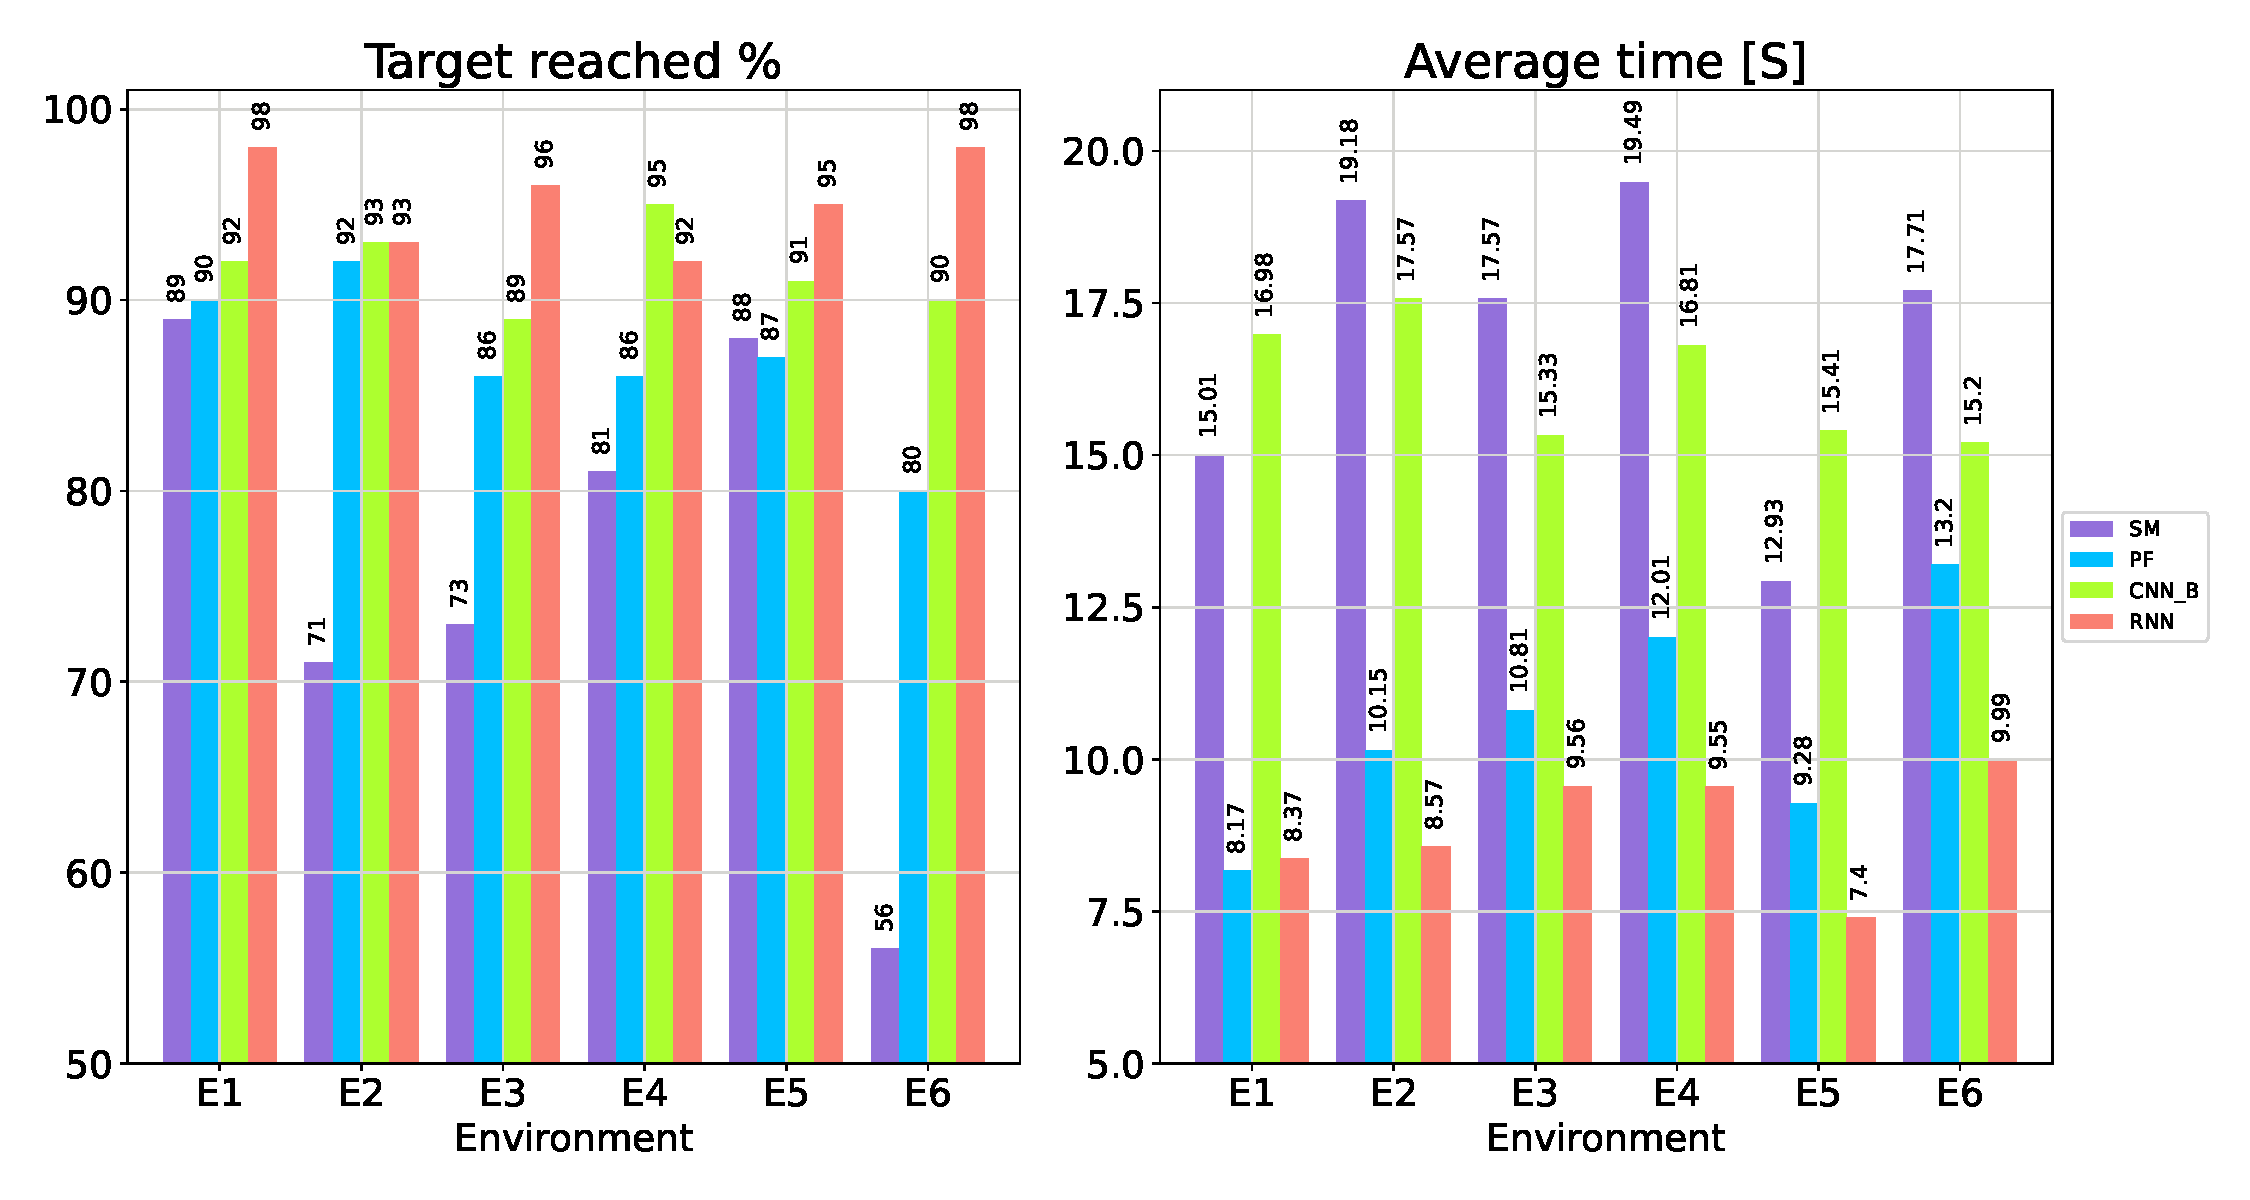
\includegraphics[width=1.0\textwidth]{images/res1_tg_time.pdf}
\caption{Successful target reach percentage (Left) and average time to reach a goal (Right). Environments with previous knowledge (training, parameters adjustment): FSM (E4), PF (E2), CNN and RNN (E1, E2, E3).}
\label{fig:res1_tg-time}
\end{figure*}

\begin{figure*}[!htbp]
\centering
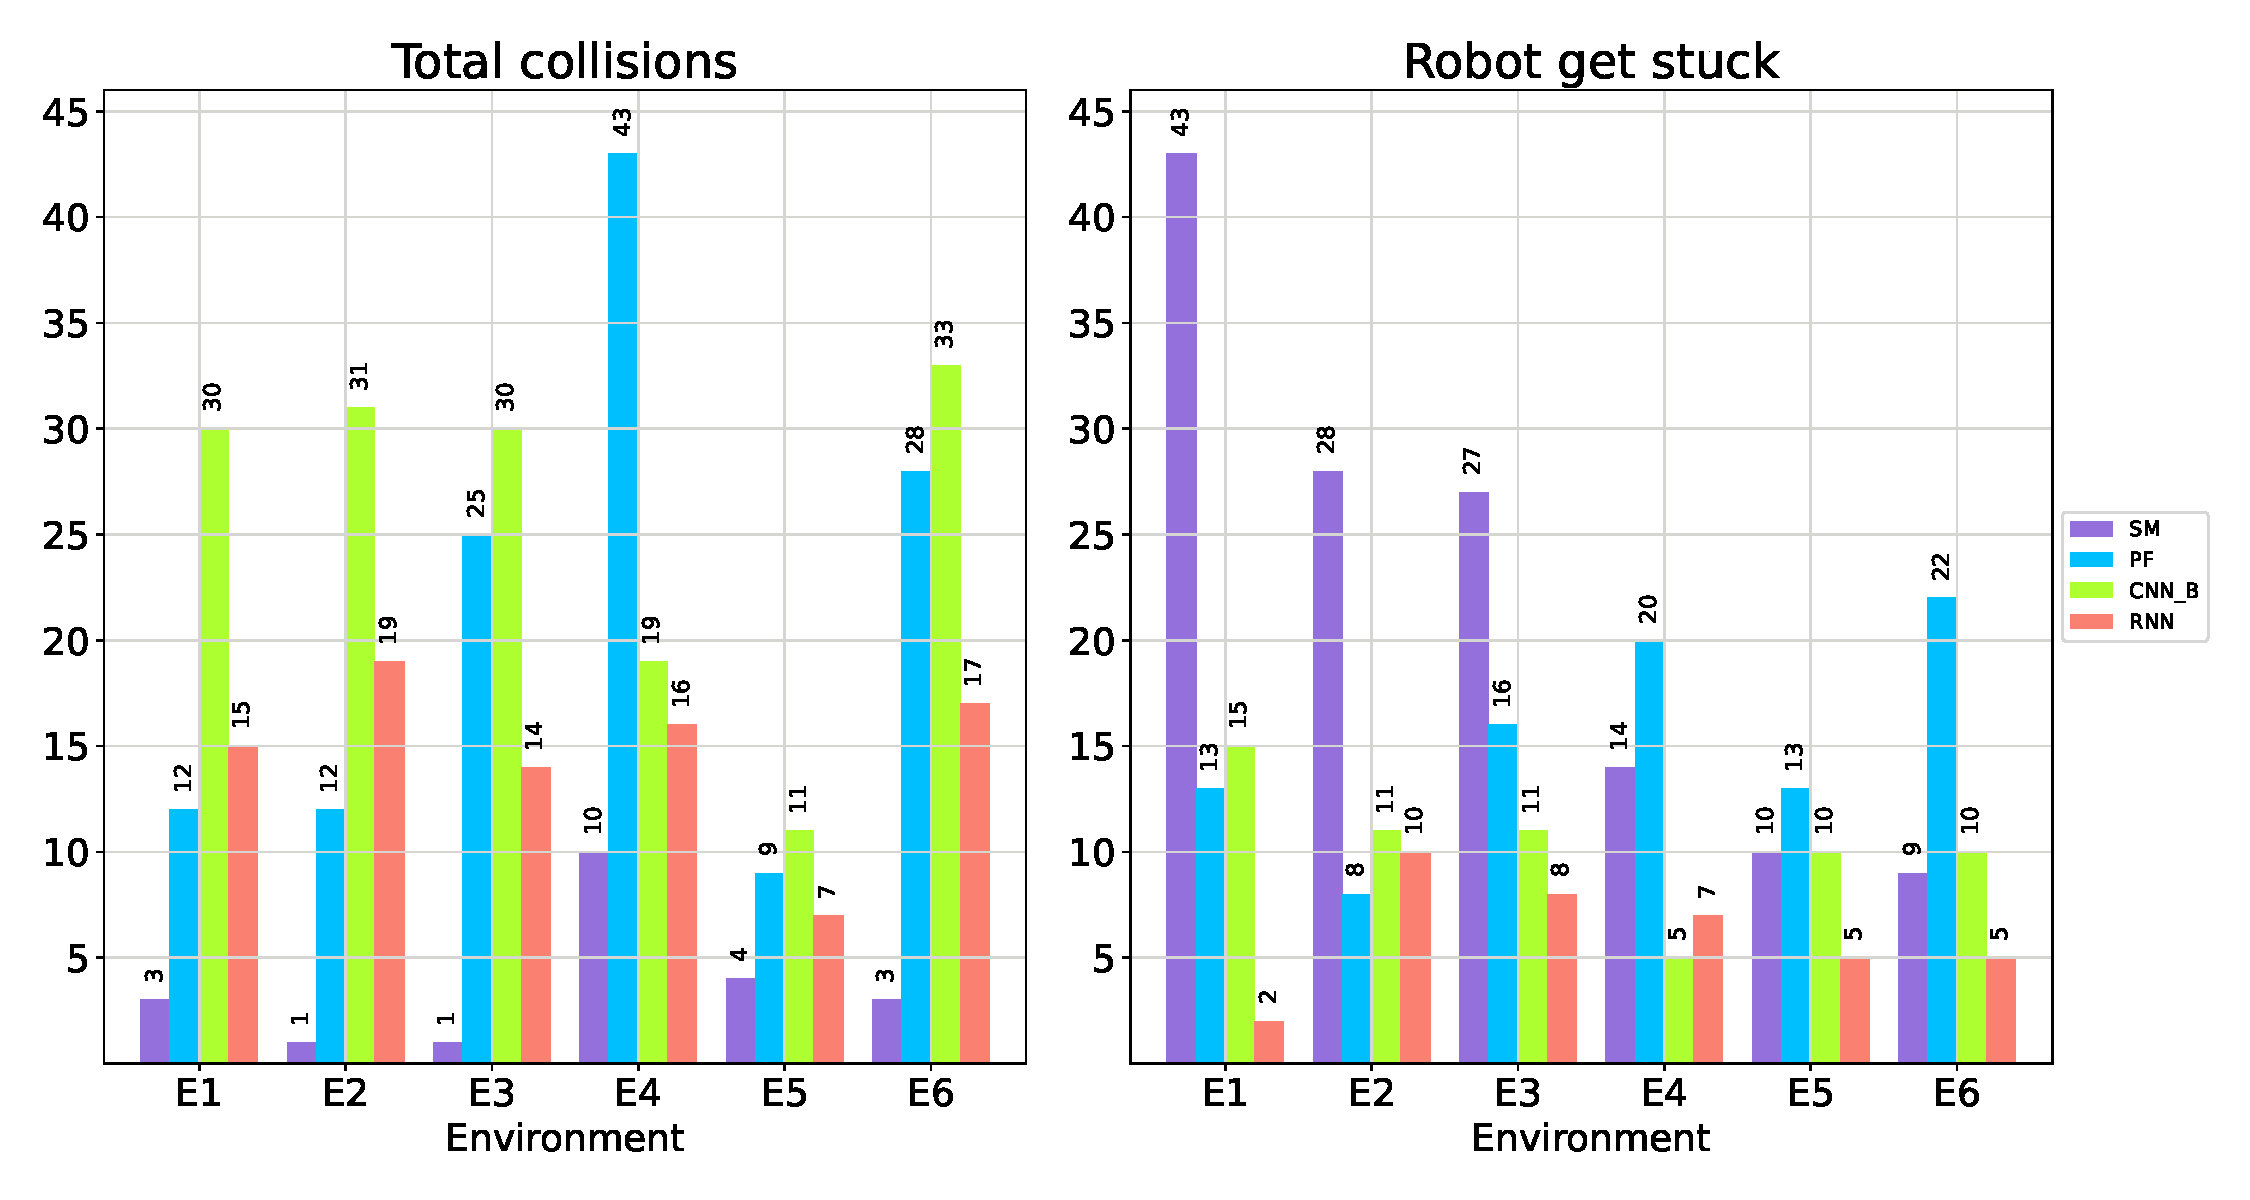
\includegraphics[width=1.0\textwidth]{images/res2_col_stuck.pdf}
\caption{Collisions occurrences (Left) and failures (Right), considering not arriving on time or getting stuck by collision.}
\label{fig:res2_col-stuck}
\end{figure*}

\section{Results}\label{sec:Results}

A direct comparison with the Pumas Navigation System (PNS) highlights the limitations of map-based approaches when operating outside their training conditions. As shown in Table~\ref{tab:nav_system}, the PNS achieves a high success rate of 98\% in the known environment (E1), where an accurate map is available. This confirms the effectiveness of classical navigation pipelines when reliable prior information is provided.

However, when deployed in an unseen environment (E4) while still relying on the map from E1, performance drops drastically to a 26\% success rate, accompanied by a significant increase in collisions. Despite the use of potential fields for local obstacle avoidance, the mismatch between the assumed map and the actual environment leads to incorrect path planning decisions and unsafe behaviors.

\textcolor{red}{The environment similarity metric in Section~\ref{sec:metric_definition} provides a quantitative comparison of map geometry, but it does not by itself explain the PNS failure. In fact, E01 and E04 appear among the ten most structurally similar pairs, with a reported distance of 0.0350 in Table~\ref{tab:most_similar}. Therefore, the low PNS success rate in E4 when using the E1 map should be interpreted as evidence of sensitivity to map mismatch in this particular experiment, not as a direct consequence of a large value of the proposed metric. A relationship between environmental distance and navigation outcomes requires additional experiments.}

These results demonstrate a fundamental limitation of map-based navigation systems: their strong dependence on accurate and up-to-date environmental representations. Even when environments share similar geometric properties, small discrepancies—such as furniture placement or corridor structure—can severely degrade performance. \textcolor{red}{In contrast, our mapless approaches generate velocity commands directly from the LOM and the relative target vector, allowing the robot to respond to environmental changes without requiring a global geometric map, global path planning, or global localization.}

Building on this comparison, we evaluate all navigation methods across both known and unknown environments. Our learning-based models, particularly the RNN (Subsection~\ref{subsec:rnn_arq}), consistently outperform traditional reactive methods such as finite state machines (FSM), which rely on predefined rules, and potential fields (PF), which are prone to local minima and reactive-only behaviors. These results confirm that the primary advantage of the proposed approach lies in its ability to generalize robustly to previously unseen environments.

During navigation, all collisions were counted, as they may briefly slow the robot, cause it to become stuck, or delay its arrival at the goal. These events provide insight into the robot’s stability and adaptability in dynamic, cluttered environments. The success rate, defined as the proportion of goals reached within a fixed time limit, is reported in Figure~\ref{fig:res1_tg-time} (Left). The corresponding average time to reach each goal is shown in Figure~\ref{fig:res1_tg-time} (Right), offering a measure of efficiency for each method. Across all tested environments, collisions, instances of the robot becoming stuck, and failures to reach targets within the time limit were observed, reflecting the challenges posed by complex layouts and narrow pathways. A summary of these events is presented in Figure~\ref{fig:res2_col-stuck}.

To complement these quantitative measures, we generated heatmaps that provide a spatial visualization of the robot’s performance in each environment. These heatmaps are derived from the recorded collision and getting‑stuck events summarized in the corresponding figures. They serve as a complementary visual aid rather than a standalone quantitative metric, allowing for a qualitative identification of areas where each navigation method faced particular challenges. In the maps, red regions correspond to zones with a high frequency of collisions and getting stuck; for FSM, red areas also include locations near doors where the robot frequently exited the map boundaries. Orange regions indicate areas where the robot experienced difficulties, such as maneuvering close to obstacles or through tight turns, and yellow regions mark zones with low collision frequency but slight issues in aligning toward the target. Comparing heatmaps across methods—FSM (Figure~\ref{fig:SM_complx}), PF (Figure~\ref{fig:PF_complx}), CNN (Figure~\ref{fig:CNN_complx}), and RNN (Figure~\ref{fig:RNN_complx})—clearly shows how learning-based approaches reduce collisions, avoid local minima, and maintain more consistent trajectories, even in unfamiliar environments.

\begin{figure*}[!htbp]
\centering
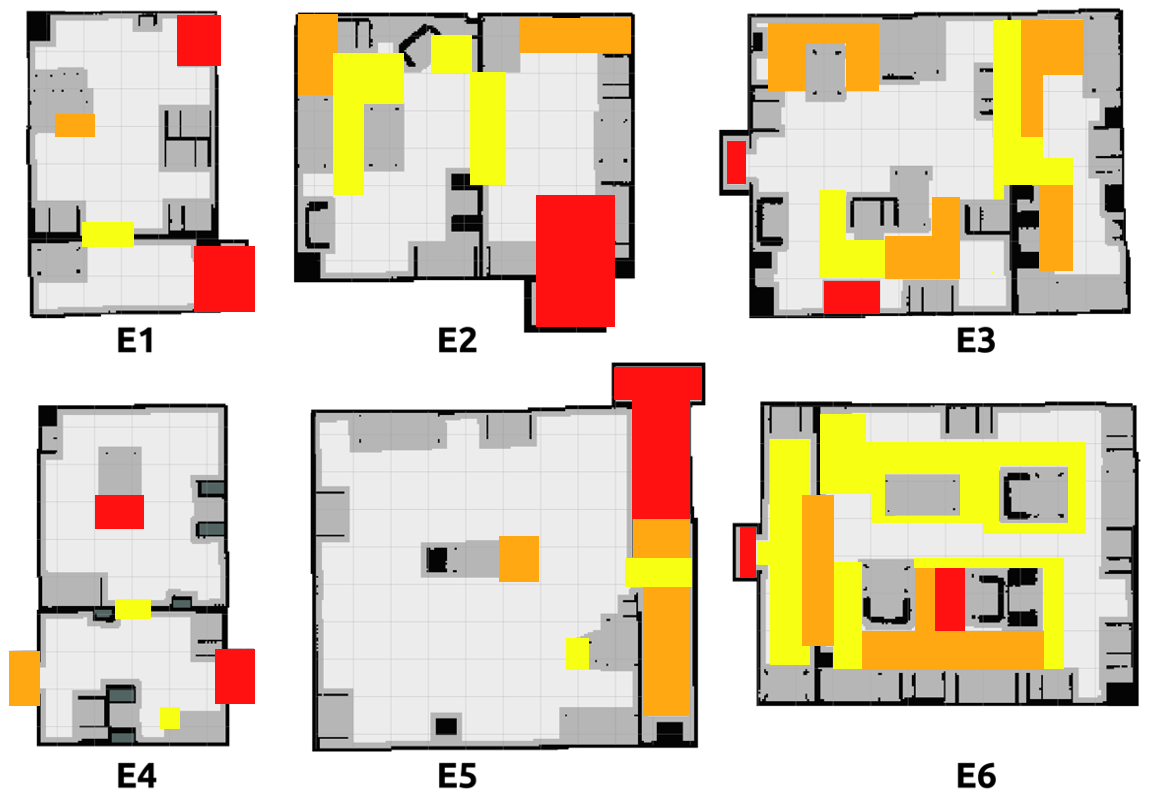
\includegraphics[width=0.85\textwidth]{images/SM_complex.png}
\caption{State machine (FSM) heat map behavior. Parameter Selection E4.}\label{fig:SM_complx}
\end{figure*}

\begin{figure*}[!htbp]
\centering
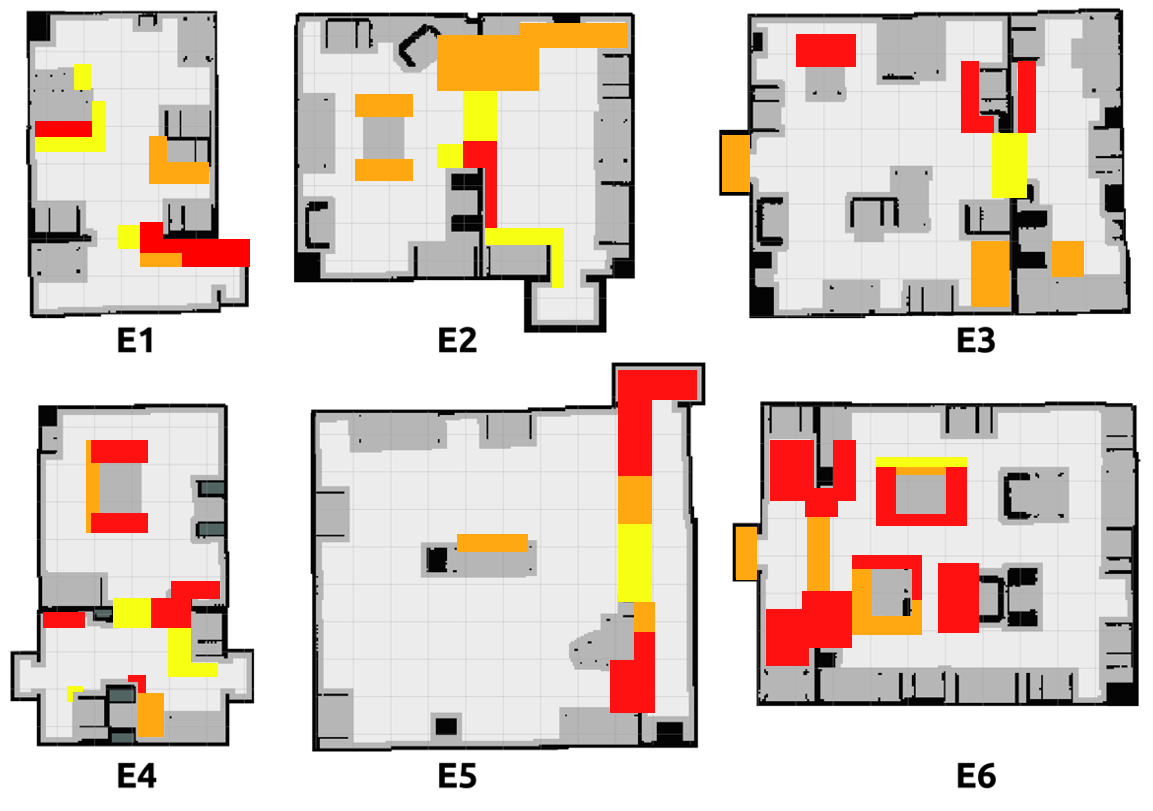
\includegraphics[width=0.85\textwidth]{images/PF_complex.png}
\caption{Potential fields (PF) heat map behavior. Constant Tuning E2.}\label{fig:PF_complx}
\end{figure*}

\begin{figure*}[!htbp]
\centering
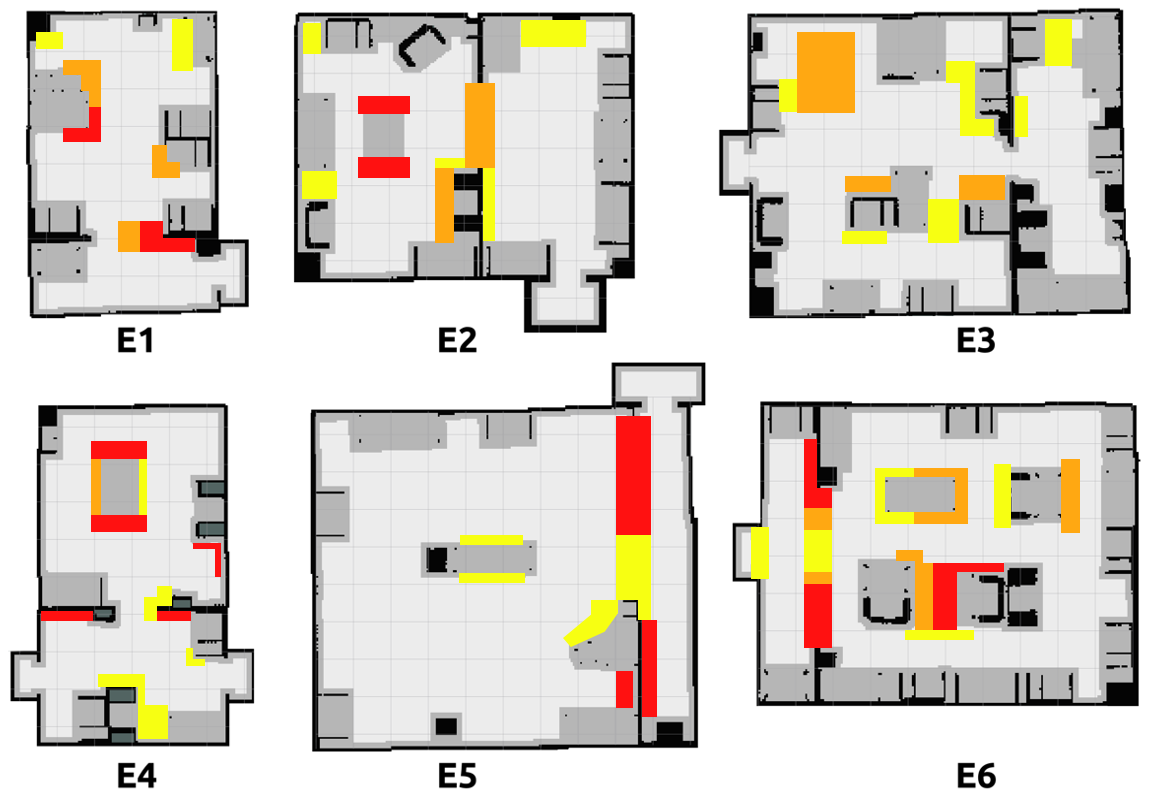
\includegraphics[width=0.85\textwidth]{images/NN_complex.png}
\caption{Convolutional neural network (CNN) heat map behavior. Training E1, E2, and E3.}\label{fig:CNN_complx}
\end{figure*}

\begin{figure*}[!htbp]
\centering
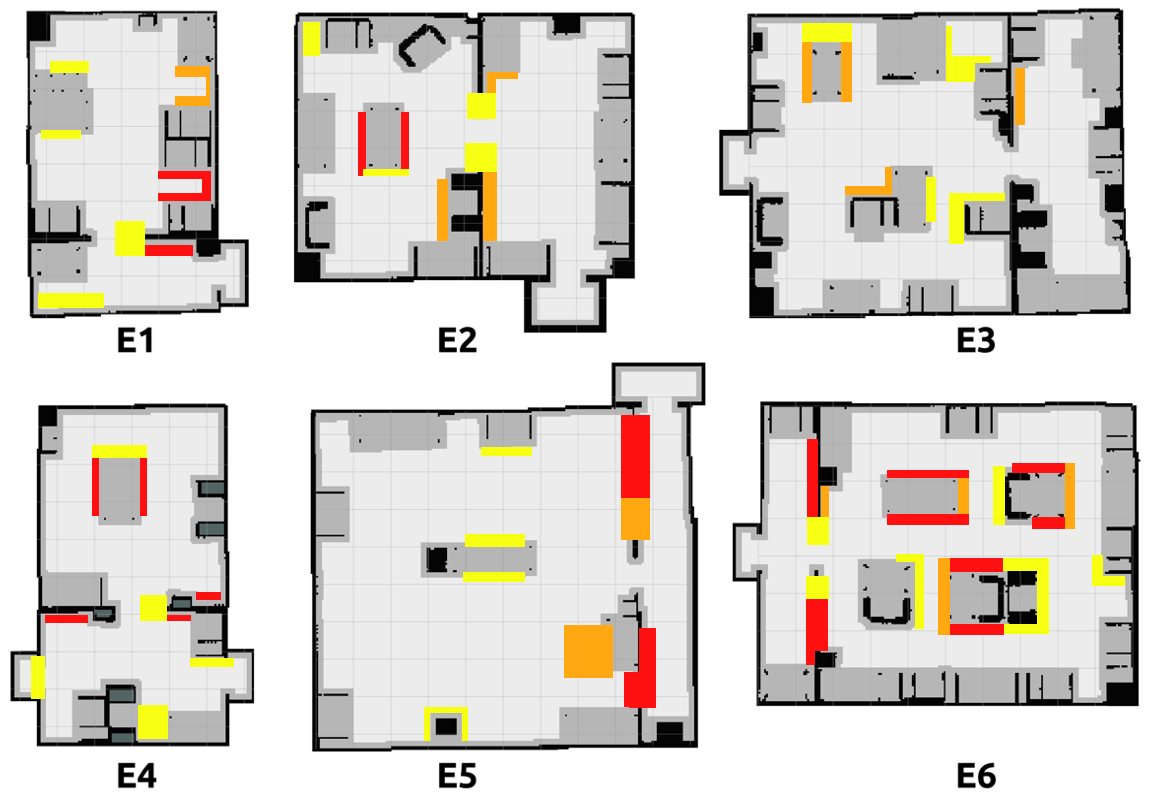
\includegraphics[width=0.85\textwidth]{images/RNN_complex.png}
\caption{Recurrent neural network (RNN) heat map behavior. Training E1, E2, and E3.}\label{fig:RNN_complx}
\end{figure*}

\section{Conclusions}\label{sec:Conclusion}

We proposed two neural network architectures for generating local navigation behaviors with obstacle avoidance: a convolutional neural network (CNN) and a recurrent variant (RNN) with four recurrent layers (see Subsections~\ref{subsec:cnn_arq} and~\ref{subsec:rnn_arq}). Unlike traditional methods—where map-based approaches may fail without an accurate or updated map—our models do not require retraining or parameter tuning, \textcolor{red}{allowing them to generate navigation commands without a global geometric map of the test environment.} In comparison, classical reactive approaches such as Potential Fields (PF) and Finite State Machines (FSM) often rely on hand-tuned parameters and may fail in unknown settings. Although the PNS performs better in a known environment (E1), its performance drops significantly in an unseen environment (E4) when using the same map, highlighting that our main contribution is robust generalization rather than superior performance in familiar scenarios.

Our experiments evaluated all methods in both previously known and unknown environments. The RNN models demonstrated strong generalization, achieving high success rates, fewer robot stuck events, and more efficient navigation than traditional approaches. Heatmaps of navigation behavior revealed specific areas where collisions or difficulties occurred, highlighting the robustness and adaptability of our learning-based models in dynamic, cluttered environments. Among the two architectures, the RNN consistently outperformed the CNN in most metrics, likely due to its ability to incorporate temporal context into decision-making.

\textcolor{red}{Furthermore, we introduced and evaluated an environment similarity metric based on entropy-regularized optimal transport. The pairwise analysis across 30 environments showed a broad range of distances, stable rankings under the tested sampling densities, and sensitivity to physical scale. These results support the use of the metric to characterize geometric differences between environments. Its ability to predict navigation performance remains to be established by correlating the distances with outcomes from controlled navigation experiments.}

A key challenge remains in heuristically generating a suitable dataset that maximizes performance across diverse environments. Nevertheless, the results indicate that learning-based navigation strategies offer a reliable, scalable, and flexible alternative to traditional rule-based methods, particularly in scenarios where prior knowledge of the environment is limited or unavailable.

\authorcontributions{D. Vanegas: conceptualization, methodology, software, writing – original draft. M. Negrete: validation, formal analysis, writing – review \& editing. J. Savage: writing and methodology review, supervision.}

\funding{This work was partially supported by UNAM-DGAPA under grant IN118226.}

\institutionalreview{Not applicable.}

\informedconsent{Not applicable.}

\dataavailability{The datasets generated during the current study are available from the corresponding author on reasonable request.}

\acknowledgments{Not applicable.}

\conflictsofinterest{The authors declare no conflicts of interest.}

\abbreviations{Abbreviations}{
The following abbreviations are used in this manuscript:
\begin{tabular}{@{}ll}
CNN & Convolutional Neural Network \\
RNN & Recurrent Neural Network \\
LOM & Local Obstacle Matrix \\
PNS & Pumas Navigation System \\
FSM & Finite State Machine \\
PF & Potential Fields \\
DSR & Domestic Service Robot \\
MSE & Mean Squared Error \\
EMD & Earth Mover's Distance \\
\end{tabular}
}

% Bibliography
\bibliography{sn-bibliography}

\end{document}